\documentclass[15pt]{article}
\usepackage{times} 
\usepackage[utf8]{inputenc}
\usepackage[spanish]{babel}
\usepackage[margin=2.5cm]{geometry}
\usepackage{graphicx}
\usepackage[export]{adjustbox}
\usepackage{caption}
\usepackage{subcaption}
\usepackage{float}
\usepackage{fancyhdr}
\pagestyle{fancy}
\fancyhead{} % clear all header fields
\fancyhead[R]{\textbf{TFM: Estudio práctico de técnicas de ofuscación y contramedidas aplicables}}
\fancyfoot{} % clear all footer fields
\fancyfoot[R]{\thepage}
\fancyfoot[L]{
\includegraphics[width=0.75cm,valign=c]{images/freyja.png}
       \href{https://github.com/drkrysSrng/freyja}{@drkrysSrng/freyja}}

\usepackage{hyperref} 
\usepackage{amsmath}
\usepackage{xcolor}
\definecolor{verde}{rgb}{0.25,0.5,0.35}
\definecolor{jpurple}{rgb}{0.5,0,0.35}
\definecolor{darkgreen}{rgb}{0.0, 0.2, 0.13}
\usepackage{listings}
\renewcommand\lstlistingname{Código}
\renewcommand{\lstlistlistingname}{Código Fuente}
\newcommand{\estiloR}{
	\lstset{ %
		language=R,                     % the language of the code
		basicstyle=\footnotesize,       % the size of the fonts that are used for the code
		numbers=left,                   % where to put the line-numbers
		numberstyle=\tiny\color{gray},  % the style that is used for the line-numbers
		stepnumber=1,                   % the step between two line-numbers. If it's 1, each line
		% will be numbered
		numbersep=5pt,                  % how far the line-numbers are from the code
		backgroundcolor=\color{white},  % choose the background color. You must add \usepackage{color}
		showspaces=false,               % show spaces adding particular underscores
		showstringspaces=false,         % underline spaces within strings
		showtabs=false,                 % show tabs within strings adding particular underscores
		frame=single,                   % adds a frame around the code
		rulecolor=\color{black},        % if not set, the frame-color may be changed on line-breaks within not-black text (e.g. commens (green here))
		tabsize=2,                      % sets default tabsize to 2 spaces
		captionpos=b,                   % sets the caption-position to bottom
		breaklines=true,                % sets automatic line breaking
		breakatwhitespace=false,        % sets if automatic breaks should only happen at whitespace
		title=\lstname,                 % show the filename of files included with \lstinputlisting;
		% also try caption instead of title
		keywordstyle=\color{blue},      % keyword style
		commentstyle=\color{darkgreen},   % comment style
		stringstyle=\color{red},      % string literal style
		escapeinside={\%*}{*)},         % if you want to add a comment within your code
		morekeywords={*,...}          % if you want to add more keywords to the set
}}

\title{TFM. Estudio práctico de técnicas de ofuscación y contramedidas aplicables.}
\author{Maria del Carmen San José}
\date{\today}

\begin{document}
	
	\thispagestyle{empty}
	
	\begin{figure}[ht]
		\minipage{0.50\textwidth}
		
\includegraphics[width=4cm]{images/logo.png}
		\endminipage
		\minipage{0.50\textwidth}
		
\includegraphics[width=8cm]{images/logo_uni.png}
		\endminipage
	\end{figure}
	
	\begin{center}
		\vspace{0.5cm}
		\LARGE
		MÁSTER EN ANÁLISIS DE MALWARE, REVERSING Y BUG HUNTING
		
		\vspace{0.8cm}
		\centering
		
\includegraphics[width=7cm]{images/front1.jpeg}
		
		
		\vspace{0.5cm}
		\LARGE
		Universidad Católica de Murcia\\
		ENIIT - Campus Internacional de Ciberseguridad
		
		
		\vspace{0.5cm}	
		\Large
		\textbf{Estudio práctico de técnicas de ofuscación y contramedidas aplicables}
		
		\vspace{0.5cm}
		\normalsize	
		PRESENTA \\
		\vspace{.3cm}
		\large
		\textbf{María San José Seco\\ \href{https://github.com/drkrysSrng/freyja}{@drkrysSrng/freyja} }
		
		\vspace{0.5cm}
		\normalsize	
		PROFESOR \\
		\vspace{.2cm}
		\large
		\textbf{David García}
		
		\vspace{0.5cm}
		\normalsize	
		ASIGNATURA \\
		\vspace{.2cm}
		\large
		\textbf{Trabajo de Fin de Máster}
		
		\vspace{0.5cm}
		\today
	\end{center}
	
	\newpage
	\tableofcontents
	\newpage
	
	\section{Introducción}
	\subsection{En qué consiste la ofuscación}
	Tanto para proteger la propiedad intelectual o intercambiar secretos, además de prevenir la ingeniería inversa de una aplicación software, el código fuente se suele ofuscar.
	
	Una forma de ofuscación es cambiar parte del código fuente, para dificultar su lectura, comprensión y su análisis. Un ofuscador es una herramienta que convierte el código fuente de un programa en otro código distinto que hace lo mismo pero de una forma mucho más difícil de leer y entender.
	
	Además, también es una de las muchas formas que tiene el malware para evadir el análisis estático o para evitar ser detectado por los métodos tradicionales anti-malware que se basan en hashes o firmas y strings para su detección.
	
	Los antivirus tradicionales hacen sus análisis para detectar el malware, normalmente comparando el hash del fichero que están analizando con los hashes que tienen en sus Base de Datos, en el caso de un analista, sería por ejemplo, compararlo con los hashes en las bases de \href{https://www.virustotal.com/gui/}{VirusTotal} \cite{virustotal}. 
	
	Otro método de análisis de código suele basarse en analizar strings. Consiste en buscar y analizar strings legibles de texto (en ASCII o Unicode) en un fichero que puede que no tenga caracteres legibles, porque sea un binario, por ejemplo. Esos strings de texto, pueden mostrarnos nombres de ficheros, IPs, URL, peticiones HTTP, claves de registro u otras cadenas que nos puedan indicar cómo funciona dicho malware. 
	
	Herramientas como YARA permiten realizar búsquedas programáticas sobre texto con el fin de realizar detecciones basadas en reglas. En el siguiente ejemplo, tenemos una regla YARA que busca tres patrones de texto\cite{yara}:
	
	\begin{figure}[h]
		\centering
		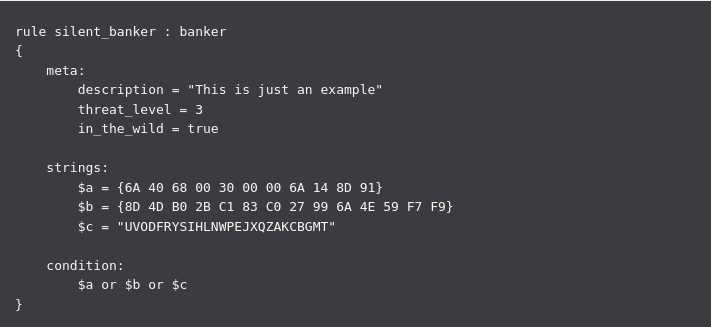
\includegraphics[width=10cm]{images/yara.png}
		\caption{Ejemplo de reglas Yara para buscar tres Strings}
	\end{figure}
	
	
	\newpage
	\section{Diagrama evolutivo del malware}
	\textbf{Fuente:} \textit{Metamorphic Malware and Obfuscation -A Survey of Techniques, Variants and Generation Kits} \cite{techniques}
	
	\begin{figure}[h]
		\centering
		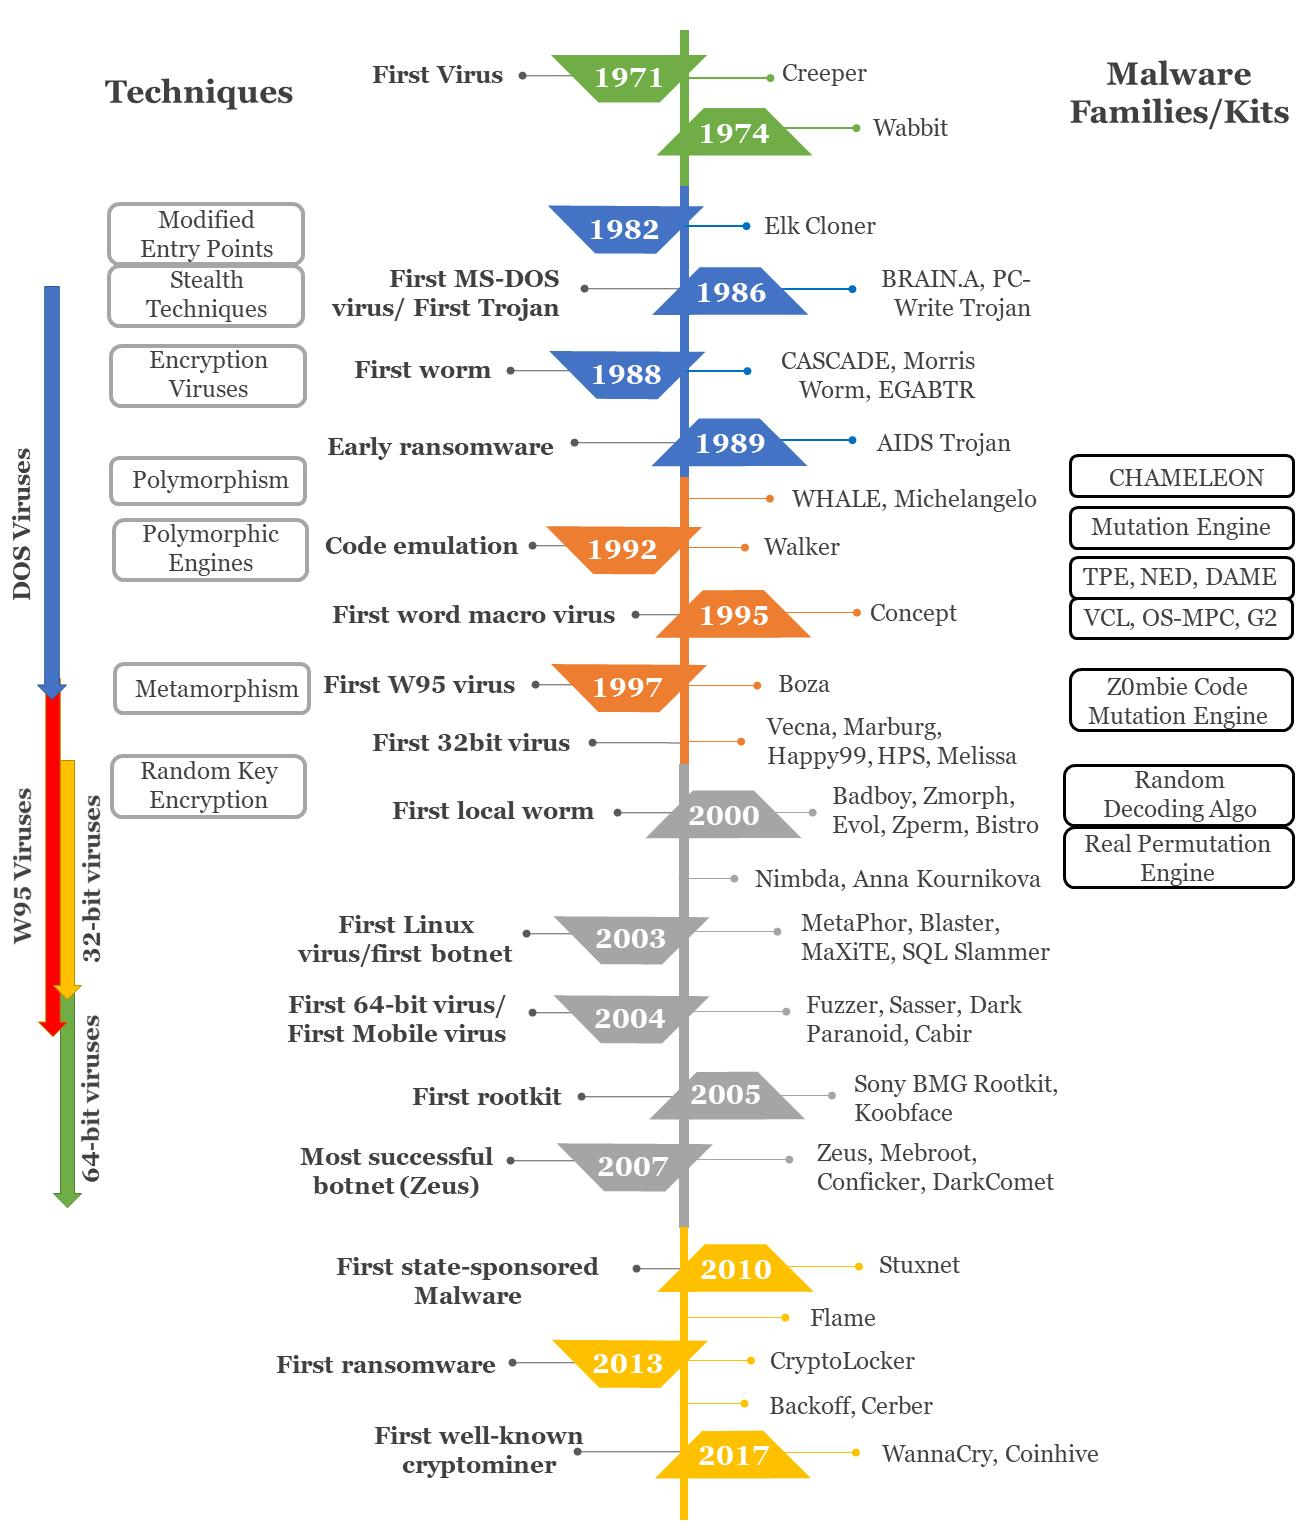
\includegraphics[width=14cm]{images/history.jpeg}
		\caption{Diagrama histórico del las variantes del malware, técnicas y motores de mutación. }
	\end{figure}

	\newpage

	\section{Tipos de Ofuscación de malware}
	\subsection{Packing}
	Se comprime el fichero para que tenga una firma distinta al original. Además de eso, los strings también serán incomprensibles. También puede incluso comprimirse el binario con software para hacerlo más pequeño. El ejecutable comprimido se empaca dentro del código requerido para descomprimirlo en tiempo de ejecución, luego la ejecución se hace en memoria. Este tipo de ofuscación lo utilizan malware como Redline Stealer \cite{redlinestealer} y Hancitor \cite{hancitor}
	
	Sin embargo, el hecho de que un programa esté empaquetado, ya es sospechoso, por lo que el malware moderno cada vez utiliza menos este sistema para pasar desapercibido.
	
	
	\subsection{Inserción de Dead-Code o código basura}
	Es una forma simple de cambiar la apariencia del programa y su funcionalidad. \textbf{\textit{NOP}} es un ejemplo de comando en ensamblador. El código original se ofusca fácilmente insertando instrucciones \textbf{\textit{NOP}}. Los análisis basados en firma podrían detectarlo simplemente eliminando esta instrucción. \footnote{NOP significa en x86 o en intel \textit{no operation}}
	
	\textbf{\textit{NOP}} no hace nada. La ejecución continúa en la siguiente instrucción. Ningún registro ni flag es afectado por eta instrucción, simplemente se genera un delay en la ejecución o una reserva de espacio en memoria.
	
	También, podemos ver encadenamiento de instrucciones como if-else o inserción de código basura que no afecta al funcionamiento del programa.
	
	\begin{scriptsize}
		\estiloR
		\begin{lstlisting}[caption={Ejemplo de Inserción de Dead-Code}, language={[x86masm]Assembler}]
			; Before obfuscation
			xor eax, eax
			move eax, 0x2D
			mov ecx, 0xA
			; After obfuscation
			xor eax, eax
			move eax, 0x2D
			nop
			nop
			mov ecx, 0xA
		\end{lstlisting}
	\end{scriptsize}
	
	
	\subsection{XOR} 
	Este método es bastante popular para ocultar datos y que no puedan ser analizados. Lo que hace es intercambiar los contenidos de dos varibles dentro del código, como por ejemplo:
	
	\begin{scriptsize}
		\estiloR
		\begin{lstlisting}[caption={Ejemplo de XOR}, language={[x86masm]Assembler}]
			XOR EBX, EAX
			XOR EAX, EBX
			XOR EBX, EAX
		\end{lstlisting}
	\end{scriptsize}
	
	XOR es una forma muy sencilla de ofuscación y encriptación ya que es muy fácil volver al valor original o recuperar una variable ofuscada ya que cualquier valor \textit{xoreado} consigo mismo da 0. Veamos la tabla de operación de XOR:
	
	\begin{center}
	\begin{tabular}{ |p{1.5cm}|p{1.5cm}||p{1.5cm}|  }
	 \hline
	 \multicolumn{3}{|c|}{Operación XOR} \\
	 \hline
	  Valor 1 & Valor 2 & Resultado\\
	 \hline
	 0 & 0 & 0 \\ 
	 0 & 1 & 1 \\  
	 1 & 0 & 1 \\
	 1 & 1 & 0\\
	 \hline
	\end{tabular}
	\end{center}
	

	
	\subsection{Reasignamiento de registros}
	Es otra técnica simple que cambia registros por cada generación mientras el código del programa y su comportamiento siguen igual. En el siguiente código, se cambian los registros al inicio y se vuelven a cambiar al final, dejando la funcionalidad como estaba. El malware W95/Regswap \cite{regswap}
	\begin{scriptsize}
		\estiloR
		\begin{lstlisting}[caption={Ejemplo de Reasignamiento de registro}, language={[x86masm]Assembler}]
			; Before obfuscation
			mv eax ecx
			xor ebx, ebx
			test eax, ebx
			; After obfuscation
			mov ebx, ecx
			xor eax, eax
			test ebx, eax
		\end{lstlisting}
	\end{scriptsize}
	
	\subsection{Sustitución de Instrucciones}
	Hay una gran variedad de sustituciones que se pueden introducir. A continuación vemos un código en el que se sustituye la instrucción \textit{push eax; mov eax, ebx} con \textit{push eax; push ebx; pop eax}. Semánticamente son equivalentes pero \textit{push} y \textit{pop} es más lento que escribir directamente en el registro con \textit{mov}. Esta técnica se utiliza en el malware W95/Zmist \cite{zmist}, y también en malware avanzados como Evol, MetaPHOR \cite{metaphor}, Zperm \cite{zperm} y Avron\cite{avron}.
	\begin{scriptsize}
		\estiloR
		\begin{lstlisting}[caption={Ejemplo de sustitución de instrucciones}, language={[x86masm]Assembler}]
			; Before obfuscation
			add eax, 05H
			mov ebx eax
			; After obfuscation
			add eax, 01H
			add eax, 05H
			push ebx
			pop eax
		\end{lstlisting}
	\end{scriptsize}

	\subsection{Base64}
	Es una forma de ofuscación muy conocida. Básicamente consiste en un esquema de codificación de caracteres, con el carácter \textit{=} como padding. El afabeto incluye desde la a-z, A-Z, + / y los caracteres numéricos del 0-9. La codificación funciona encadenando 3 caracteres para generar una cadena de 24 bits, que luego se divide en cuatro fragmentos de 6 bits, cada uno de los cuales se traduce a uno de los caracteres Base64. A pesar de ser una técnica trivial, es ampliamente utilizada, sobre todo para ofuscar cadenas.
	
	
	\subsection{Transposición de Código}
	Reordena la secuencia de instrucciones del código original sin afectar el comportamiento del código. Hay dos maneras:
	\begin{itemize}
		\item Cambiar las instrucciones de forma aleatoria y luego inserta ramas incondicionales o saltos para restaurar la ejecución original. No es difícil detectar este método porque el programa original se puede restaurar eliminando las ramas incondiconales o saltos.
		\item Crear nuevo código eligiendo y reordenando las instrucciones que son independientes entre ellas, es una técnica difícil de implementar, pero hace que la detección sea más difícil.
	\end{itemize}

	\subsubsection{Reordenamiento de subrutinas}
	También conocido como Block Reordering o reordenamiento de bloques, es una técnica que reordena el flujo del proceso cambiando bloques del código que tienen subrutinas independientes. Si un código tiene n subrutinas de código, tendrá \verb*|n!| permutaciones para reordenar dicho código.
	
	\begin{scriptsize}
		\estiloR
		\begin{lstlisting}[caption={Ejemplo de sustitución de reordenamiento de subrutina}, language={[x86masm]Assembler}]
			; Before obfuscation
			mov eax , ebx
			add ecx , edx
			add eax , ecx
			
			; After obfuscation
			add ecx , edx
			mov eax , ebx
			add eax , ecx
			
		\end{lstlisting}
	\end{scriptsize}

	\begin{scriptsize}
		\estiloR
		\begin{lstlisting}[caption={Ejemplo de Code Cransposition, Subroutine Redordering and Garbage Code}, language={[x86masm]Assembler}]
			; Before obfuscation
			mov eax, ecx
			mov ebx, 10
			mul ebx
			add eax, 5
			mov ecx, eax
			; After obfuscation
			mov ebx, 10
			jmp F1
			jnk
			F2: push edx; jnk
			pop ecx
			jmp F3
			F1: mul, ebx
			add ecx, 1; jnk
			add ecx, 5
			jmp F2
			F3: mul ebx
		\end{lstlisting}
	\end{scriptsize}

	\subsection{Integración de Código}
	Fue por primera vez visto en W95/Zmist \cite{zmist}, le indica al código malicioso, unirse al código del programa objetivo, el malware decompila el programa e inyecta el código y lo reensambla para poder utilizarlo.
	
	Lo que hace este tipo de malware es buscar un fichero/comando/código o binario para inyectar código propio dentor de él, como si fuese un código parásito y luego si es necesario lo recompila. Es una forma de ofuscación muy avanzada.
	
	En el caso de Zminst, éste se inyectaba buscando instrucciones \verb*|jmp| en ficheros objetivo. Inyectando su código con una copia encriptada suya, reescribía el fichero.
	
	A continuación vemos un ejemplo de una inyección de un programa a través de una instrucción de código \verb*|jmp| \cite{parasite}

	\newpage
	\begin{figure}[h]
		\centering
		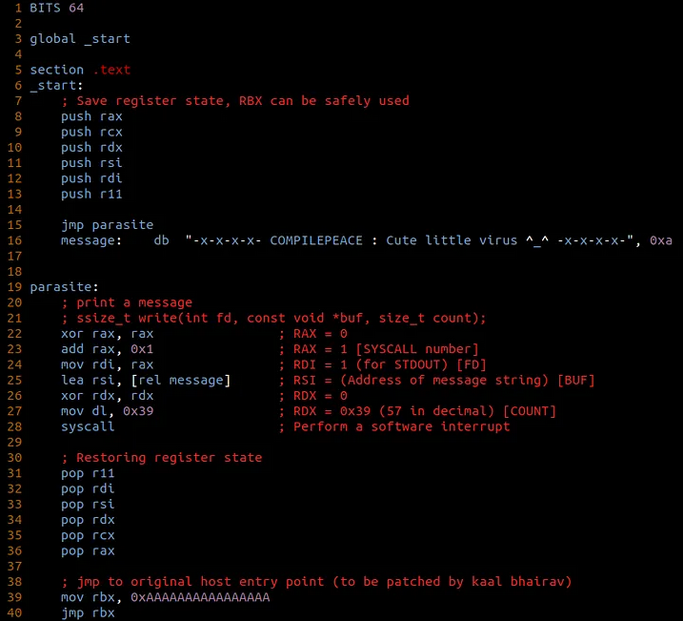
\includegraphics[width=12cm]{images/code_insertion.png}
		\caption{Ejemplo de inyección de un programa parásito }
	\end{figure}
	
	
	\newpage
	\subsection{Expresiones MBA}
	Las expresiones MBA o Mixed Boolean-Arithmetic sirven para ofuscar el código utilizando operadores booleanos o polinomios dejando la funcionalidad del código intacta. Es un método para preservar la semántica a través de transformaciones con simples expresiones, para dificultar el análisis del código. Esta técnica consiste en la mezcla de expresiones aritméticas y operaciones booleanas. El código binario con ofuscación MBA puede ocultar los datos y algoritmos de análisis estáticos y dinámicos, incluyendo los análisis avanzados. 
	
	
	\begin{scriptsize}
		\estiloR
		\begin{lstlisting}[caption={Ejemplo de expresiones MBA equivalentes}, language={python}]

			def e1(x, y):
			    return x + y
			
			def e2(x, y):
			    return (x + y) + 2 * (x & y)
			    
			print("Mba test e1 with 3 and 4 is: ", e1(3, 4))
			print("Mba test e2 with 3 and 4 is:", e2(3, 4))
			
			#Resultado:
			El resutado de e1 es:  7
			El resutado de e2 es:  7
			
		\end{lstlisting}
	\end{scriptsize}
	
	A continuación podemos ver más ejemplos de expresiones booleanas y sus equivalentes en MBA:
		\begin{figure}[h]
			\centering
			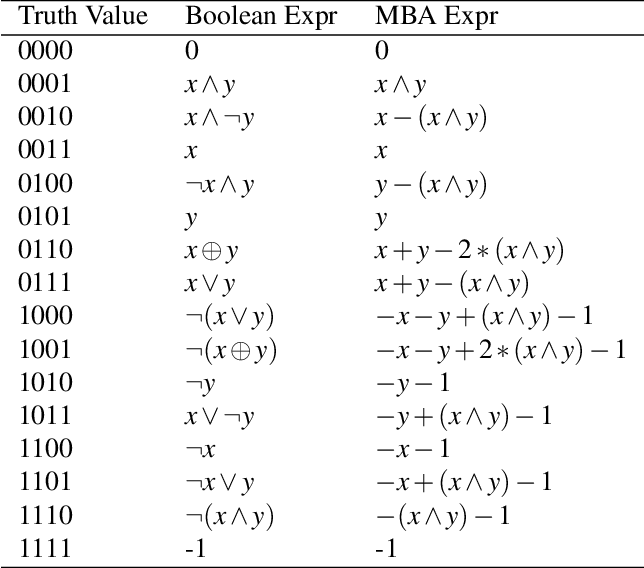
\includegraphics[width=10cm]{images/mba_table.png}
			\caption{Ejemplos de equivalencias en expresiones MBA }
		\end{figure}
	
	
	\subsection{Expresiones Opacas}
	Normalmente se refieren a expresiones que siempre toman el valor de True o False, conocidas en tiempo de compilación pero son evaluadas en tiempo de ejecución. Aquí tenemos tres ejemplos donde añadiendo este tipo de expresiones condicionales, siempre se va a ejecutar el código que nos interese:
	
	\begin{scriptsize}
		\estiloR
		\begin{lstlisting}[caption={Ejemplo de expresiones Opacas equivalentes}, language={python}]
			
			def o1(x):
			    if x % 2: # 5 cannot be divided by 2, always true
			        x = 1 << x
			        x = 2 * x + 9
			        return x
			
			def o2(x):
			    if ((4 * x * x + 4) % 19) != 0:
			        x = 1 << x
			        x = 2 * x + 9
			        return x
			
			def o3(x):
			    if ((4 * x * x + 4) % 19) != 0:
			        if x % 2:
			            x = 1 << x
			            x = 2 * x + 9
			            return x
			        else:
			            x *= 5
			            return x
			    else:
			        x += 85
			        return x
			print("Opaque test o1: ", o1(5))
			print("Opaque test o1: ", o2(5))
			print("Opaque test o1: ", o3(5))
			
			
			# Resultado
			El resutado de o1 es:  73
			El resutado de o2 es:  73
			El resutado de o3 es:  73
			
		\end{lstlisting}
	\end{scriptsize}
	
	
	\newpage
	\section{Encriptación, Compresión y Metamorfismo}
	El metamorfismo y otras formas de ofuscación, son la parte principal de las amenazas que nos encontramos hoy en día. Al igual que las técnicas basadas en firma de los antivirus avanzan, también los niveles de ofuscación empleados por los actores para evadirlas.
	
	El malware hace uso de Entry Point Obscuration (EPO) para evitar coherencia en el orden al ejecutar el archivo infectado. En este ejemplo, el encabezado apuntaría a una dirección que ejecutaría el código infeccioso que luego apuntaría al fichero host para que la ejecución del virus lo hiciera sin darse cuenta.
	
	\begin{figure}[h]
		\centering
		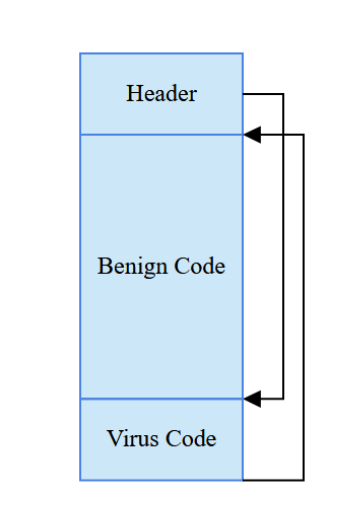
\includegraphics[width=4cm]{images/EPO.png}
		\caption{Entry Point Obscuration (EPO)}
	\end{figure}
	
	
	\subsection{Oligomorfismo}
	
	Comenzó como una forma de evadir las técnicas de escaneo basadas en firma. Para evitar esto, tenemos las técnicas de escaneo tales como Wildcard y Mismatch. Teniendo en cuenta que el código de la infección suele estar añadido a un fichero, escaneos Top-and-Tail pueden ser efectivos para extraer las firmas de alguas partes del código. Además, el uso de sandboxes o emuladores sirve para ver cómo se extrae el malware y monitorear la memoria y el código que se dumpea. El primer malware Oligomórfico fue Whale DOS \cite{whale}, identificado por primera vez en 1990. En la siguiente imagen, la rutina de desencriptado se utiliza para desencriptar el cuerpo y evitar la detección del malware.
	
	\begin{figure}[H]
		\centering
		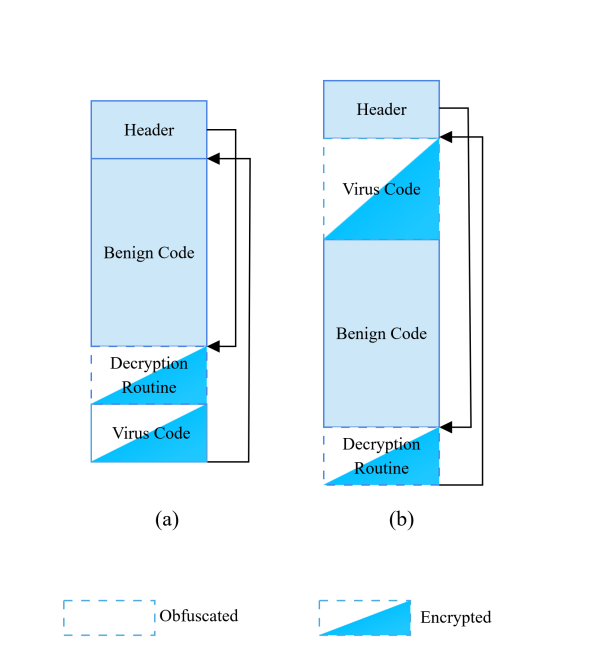
\includegraphics[width=9cm]{images/oligomorphism.png}
		\caption{Malware Oligomórfico y Metamórfico}
	\end{figure}	

	La limitación de esta técnica, es que el bucle de posibles descifradores es finito. Por ejemplo el W95/Memorial \cite{memorial} tiene exactamente 96 desencriptadores para elegir. Una vez que se agota un generador oligomórfico, la única solución es introducir ofuscación en la Rutina de Desencriptado y así tendremos una forma infinita de rutinas de desencriptado dando lugar al malware de tipo Polimórfico. Dando lugar a la primera generación de malware Polimórfico como 1260 \cite{1260} y famosos generadores como Phalcon/Skism Mass-Produced Code Generator (PS-MPC) \cite{psmpc} y Virus Creation Lab (VCL)\cite{vcl} que se siguen utilizando actualmente.
	
	\subsection{Polimorfismo}
	Este malware es capaz de desencriptar como ofuscar y recompilar todo en uno. El cuerpo dsencriptado crea un nuevo desencriptador mutado, utilizando un algoritmo aleatorio de encriptado y luego permite al desencriptador encriptar antes de linkar las dos partes. El único problema son los emuladores, la ejecución en memoria puede ser detectada por los investigadores de malware.
	Las primeras generaciones de ofuscadores tenían el siguiente problema:
	\begin{itemize}
		\item El tamaño del código infeccioso era constante (Polimer.512.A y Vienna \cite{vienna}).
		\item Adjuntando o preadjuntando al fichero objetivo, puede ser detectado por escaneo de firma.
		\item Segmentos de código similares entre generaciones del malware pueden detectarse por análisis de entropía.
	\end{itemize}

	\paragraph{Ejemplos de malware polimórfico:} 
	\begin{itemize}
		\item Luna. Uno de los primeros malware porlimórficos desarrollado por Bumblebee en España en el año 1999. Apareció en la cuarta versión de la revista 29A. \cite{luna}
		\item Loveletter. Uno de los primeros gusanos en alcanzar un gran número de daños.\cite{loveletter}
		\item Storm Worm Email. Responsable del 8\% de todas las infecciones gloables de malware. Utilizando como infección un archivo adjunto de un email. Su difícil detección era porque su código cambiaba cada 30 minutos aproximadamente. \cite{stormwormemail}
		\item CryptoWall. Es un ransomware que cifra los ficheros de la computadora de la víctima exigiendo el pago de un rescate para su descifrado. \cite{cryptowall}
		\item Virlock. Se vio por primer avez en 2014, pero en septiembre de 2016 se descubrió que era capaz de propagarse a través de las redes a través de aplicaciones de colaboración y almacenamiento en la nube. No sólo cifra los ficheros sino que también los convierte en infectador de archivos binarios polimórfico. \cite{virlock}
		\item CryptXXX. Distribuido por Angler Exploit Kit, encripta varios archivos almacenados en las unidades locales y extraíbles mediante RSA4096, generando una clave pública y otra privada. La clave privada se almacena en servidores remotos, también copia ficheros privados como cookes, datos de navegación... \cite{cryptxxx}
		\item CryptoLocker. Es un caballo de Troya que infecta la computadora y luego busca ficheros para cifrar, tanto discos duros, USB, unidades de red o en la nube. Sólo es para Windows. El cifrado es asimétrico. \cite{cryptolocker}
		\item Wannacry. Este ransomware se propaga aprovechando una vulnerabilidad en el protocolo de Windows Server Message Block (SMB). Este protocolo permite la comunicación entre máquinas Windows en red. Explotó en 2017 infectando a más de 230,000 computadoras en todo el mundo, causando daños valorados en miles de dólares. Fue difundido por EternalBlue, un exploit de Zero-Day que usa una versión antigua del protocolo SMB. Se cree que fue creado por la Agencia de Seguridad Nacional de EE.UU. (NSA) y luego obtenido por los Shadow Brokers. \cite{wannacry}
	\end{itemize}
	
	\subsection{Metamorfismo}
	Este tipo de malware introdujo la idea por primera vez la idea de que no pueden existir dos generaciones de malware con firmas similares. En el gráfico anterior (b), se muestra el virus metamórfico. A diferencia del polimorfismo, el código viral está ofuscado, estando todo el virus presente en un estado ofuscado. Esto introduce la idea de que los Metamórficos son body-Polimórficos, que como resultado no tienen el cuerpo constante. Los primeros virus de tipo metamórfico fueron W95/Regswap en 1998 \cite{regswap} seguido del W32/Ghost en el 2000 \cite{ghost}. Este último contenía 10 submódulos, 3.6 millones de posibles variaciones para hacer un reordenamiento de subrutinas. En el caso del gráfico anterior(b), la separación entre el desencriptador y el cuerpo malicioso no es posible y la ofuscación  hace que el cifrado ya no sea necesario. Además la rutina de descrifrado se encuentra en el código benigno, así que no necesita desempacar para crear un cuerpo del malware constante como en el caso del polimorfismo. Uno de los generadores metamórficos más utilizados es W32/NGVCK creado en 2001 \cite{ngvck} creado en 2001. Este tipo de malware tiene un motor de mutación que contiene muchos subprocesos.
	
	\subsection{Motor Metamórfico}
	Es el responsable de la ofuscación reconstrucción del binario para que éste funcione. Los componentes de este motor son los siguientes:
	\begin{itemize}
		\item \textbf{Disassembler:} Responsable de convertir el código binario en instrucciones de ensamblador.
		\item \textbf{Shrinker:} Eliminar la mayoría del código basura producido por generaciones anteriores o de otro código generado por ofuscación.
		\item \textbf{Permutor:} Lleva a cabo la mayoría de la ofuscación utilizando permutaciones y subrutinas, muchas veces de forma aleatoria. También hace inserción de instrucciones \textit{jmp}
		\item \textbf{Expander:} Sustituye instrucciones para convertirlas en otro conjunto de instrucciones equivalente, además los registros se reasignan y las variables se vuelven a seleccionar utilizando tablas de sustitución. Código basura y código que no hace nada se añade y las funciones se alinean.
		\item \textbf{Assembler:} Reestructura el control de flujo y reconvierte el código ensamblador otra vez al código binario donde se vuelve funcional otra vez.
		\item \textbf{Viral Code:} Contiene las instrucciones principales que se ejecutarán en todas las generaciones de malware- También contiene las instrucciones que coordina el motor de mutación y otros componentes.    
	\end{itemize}

	Los pasos de \textbf{Permutor} y \textbf{Expander} se utilizan de forma sofisticada en los W32/Zmist \cite{zmist} y W32/Etap \cite{etap}
	
	\begin{figure}[H]
		\centering
		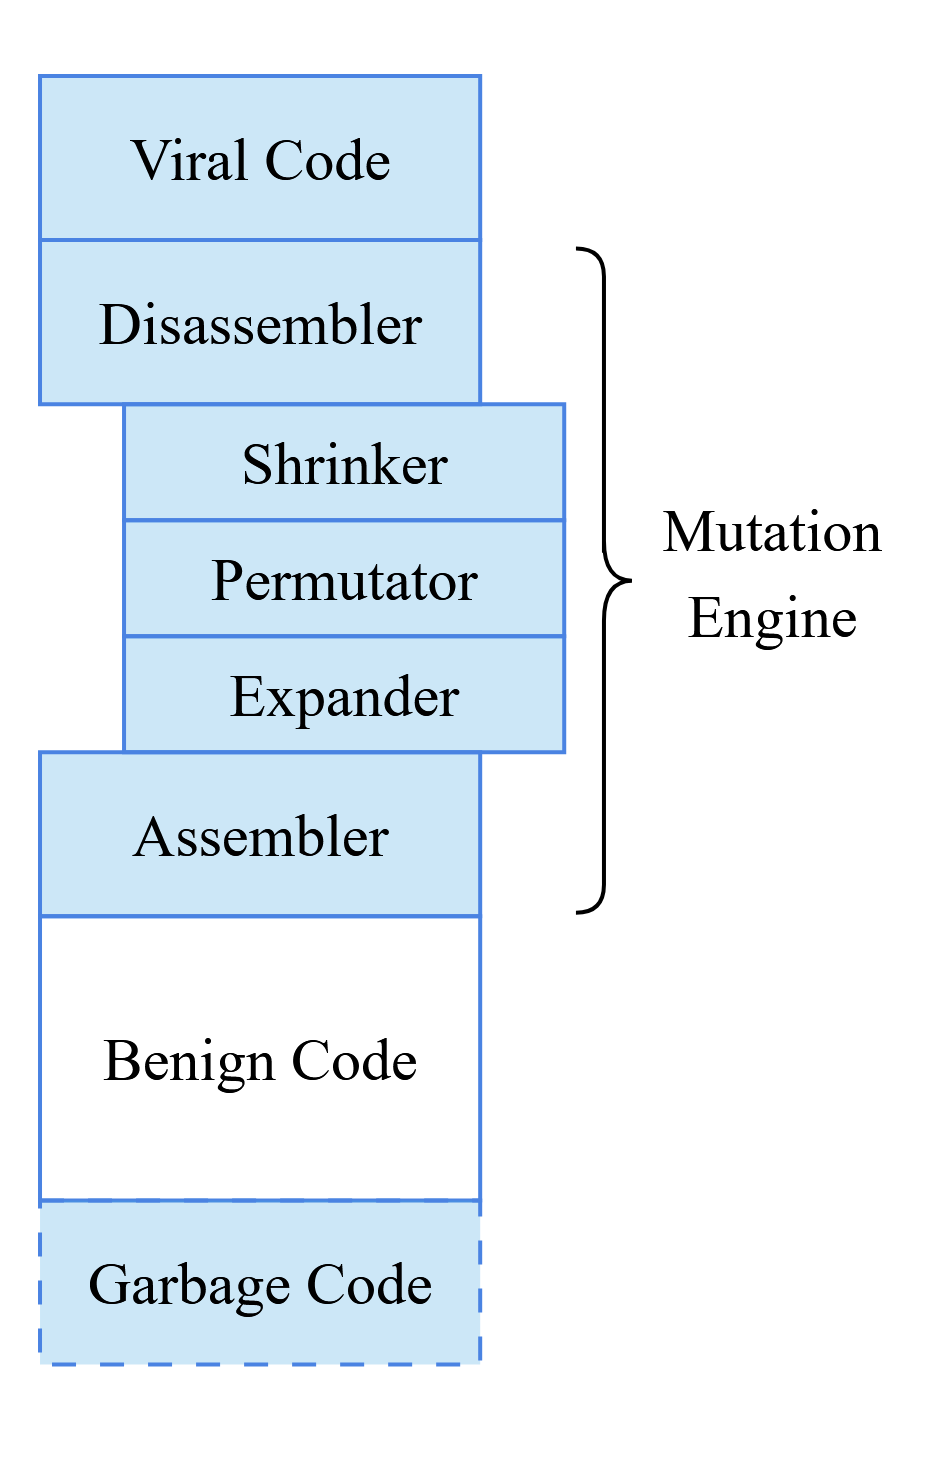
\includegraphics[width=4cm]{images/metamorphic.png}
		\caption{Componentes del Motor Metamórfico}
	\end{figure}

	\subsubsection{Pasos del Motor Metamórfico para desencriptar}
	\begin{enumerate}
		\item La rutina desencripta el cuerpo del Malware y ejecuta una instancia del mismo.
		\item La Rutina de Desencriptado desencripta el motor de mutación y lo ejecuta.
		\item El Shrinker desofusca el cuerpo del código malicioso.
		\item La ofuscación se lleva a cabo introduciendo una nueva y únca rutina de desencriptado.
		\item El cuerpo del código malicioso se ofusca por el motor de mutación para producir una generación única utilizando varias técnicas . Luego se encripta utilizando un algoritmo único, una clave estática o una clave temporal.
		\item Finalmente el motor de mutación es encriptado.
	\end{enumerate}

	\begin{figure}[H]
		\centering
		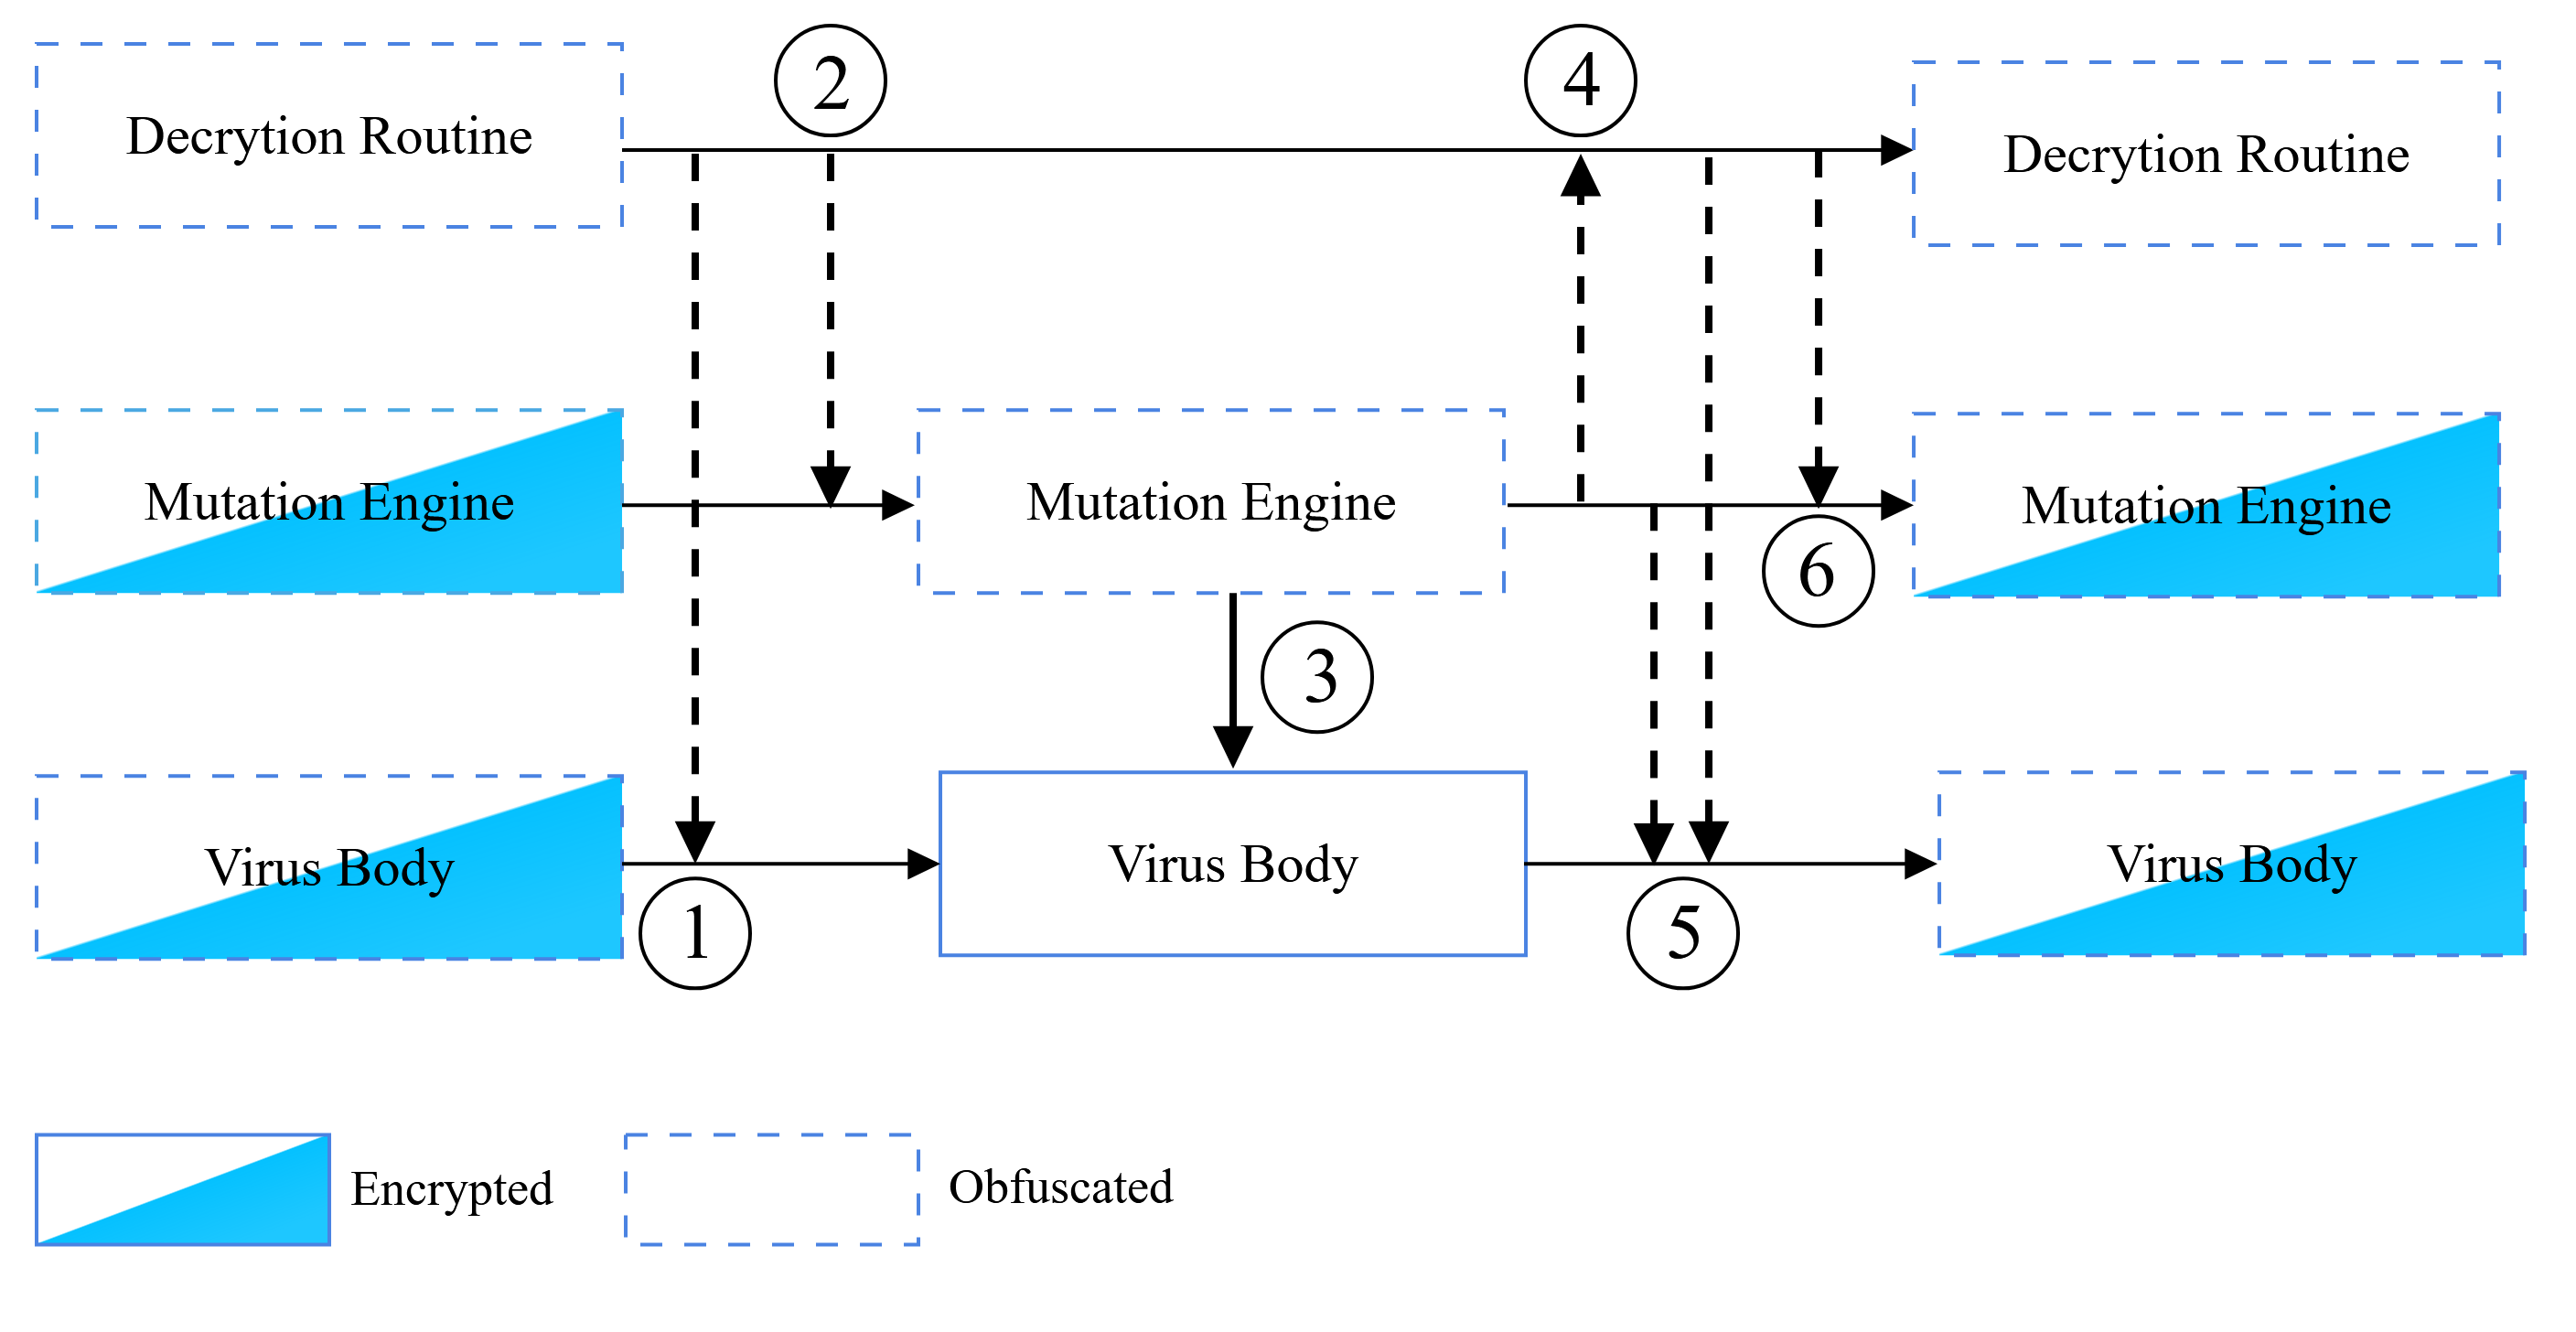
\includegraphics[width=10cm]{images/steps_metamorphic.png}
		\caption{Pasos del Motor Metamórfico para Desencriptar}
	\end{figure}
	
	\subsection{Encriptación}
	La primera forma de encriptación fue por el Malware CASCADE utilizando un simple \textit{XOR} \cite{cascade}.
	\begin{figure}[H]
		\centering
		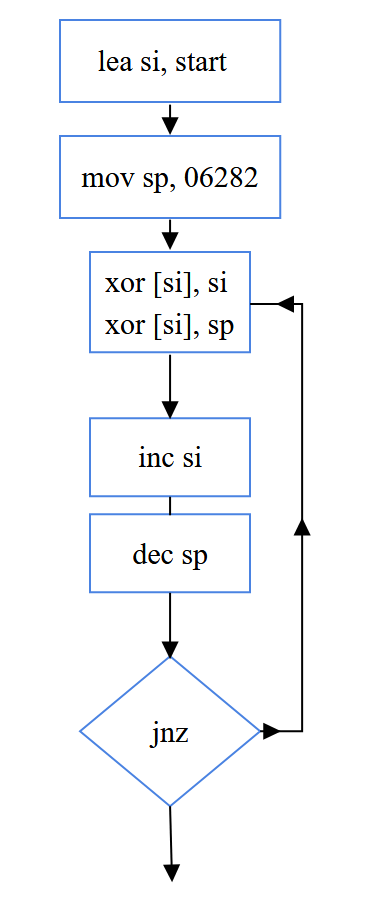
\includegraphics[width=4cm]{images/cascade.png}
		\caption{Diagrama de funcionamiento del malware CASCADE}
	\end{figure}
	Más adelante, el malware evolucionó de forma que en lugar de tener una sóla encriptación, tienen docenas de ellas, como en el caso del DOS/Whale en 1990 \cite{whale} o de forma aleatoria como en el caso de W32/MetaPHOR \cite{metaphor}
	La encriptación básica, puede desarrollarse con una única clave byte a byte, sin embargo hay formas alternativas en las que la clave se va actualizando a cada paso o incluso utilizando los caracteres encriptados.
	
	\begin{figure}[H]
		\centering
		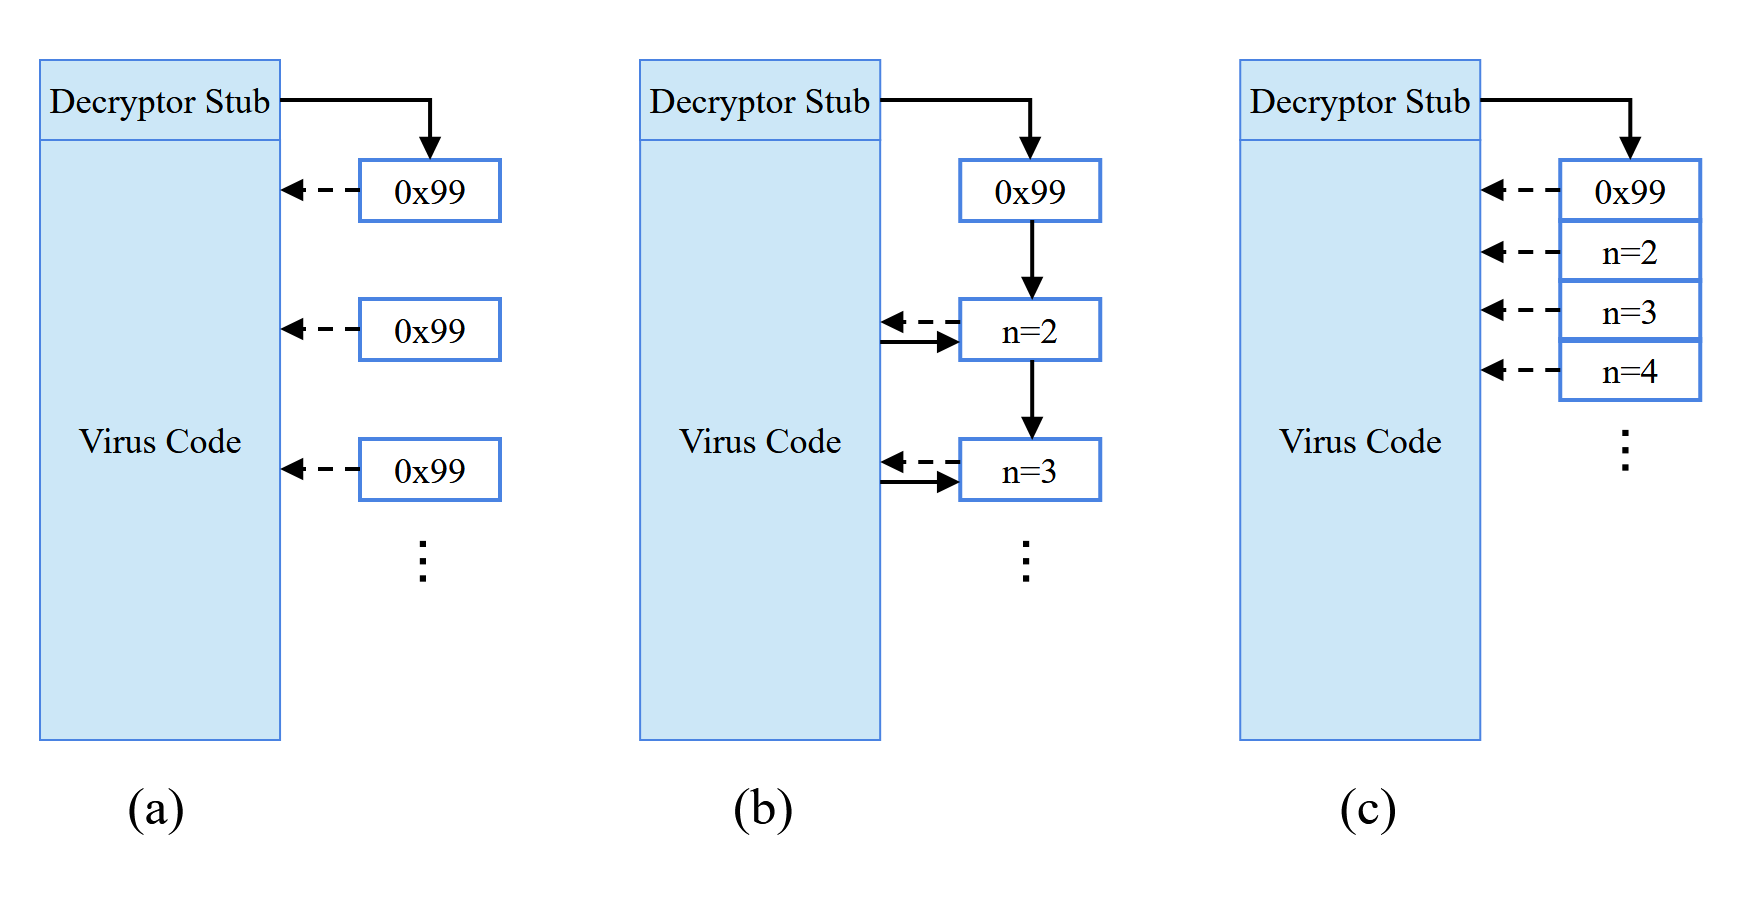
\includegraphics[width=12cm]{images/encrypt.png}
		\caption{Tipos de encriptación. a. Clave reutilizada. b. La clave va cambiando por cada bloque. c. Se utiliza el código cifrado para encriptar cada bloque}
	\end{figure}

	\subsection{Compresión}
	Representa un nivel adicional de ofuscación. Un Packer se define como una utilidad que aplica una forma de compresión al ejecutable, tanto para reducir el tamaño del fichero, evitar el análisis de entropía o introducir una capa de ofuscación en el encabezado PE. Se estima que el 80\% del malware utiliza algún tipo de empaquetador así como el 90\% de todos los gusanos.
	
	Dos de los Packer más populares son UPX \cite{upx} y ASPACK \cite{aspack}
	
	\begin{figure}[H]
		\centering
		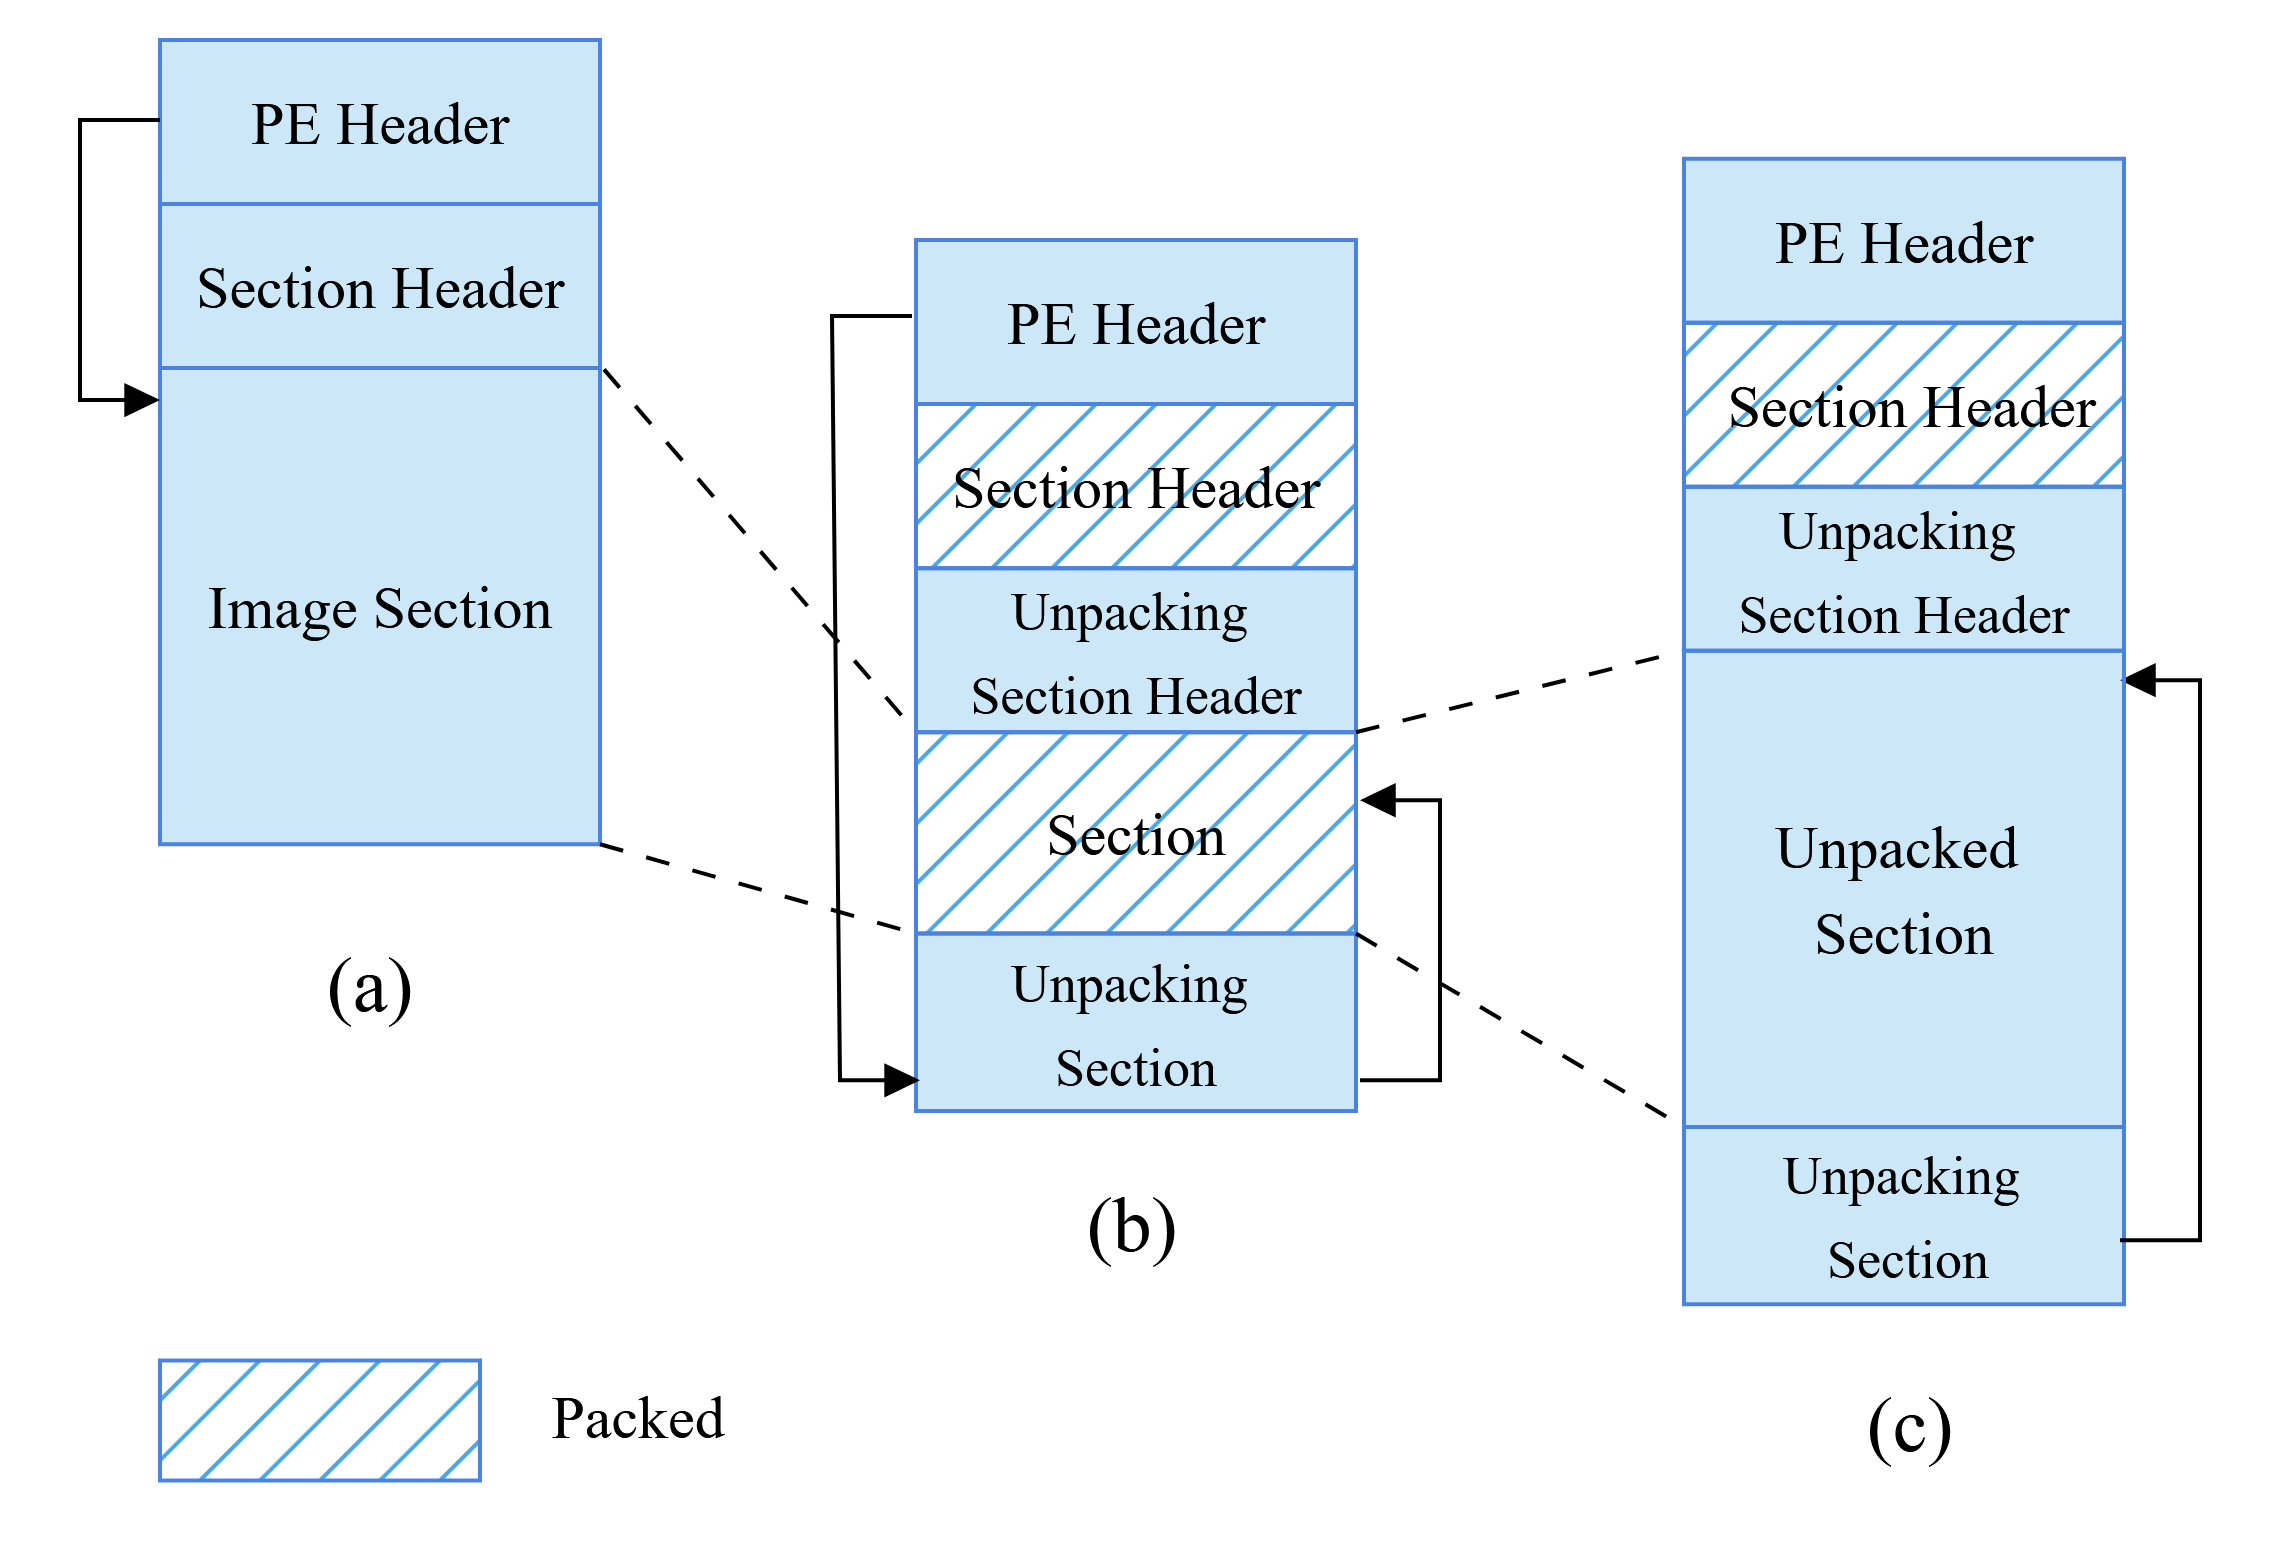
\includegraphics[width=12cm]{images/packer.png}
		\caption{Pasos en un Packer}
	\end{figure}

	
	\newpage
	\section{Análisis de Entropía\label{entropy}}
	El término científico Entropía se define generalmente como la medida de aleatoriedad o desorden de un sistema, lo cual es importante para la evasión de Antivirus. El malware suele contener código altamente randomizado, encriptado u decodificado(ofuscado) para hacer el análisis y la detección difíciles. Uno de los métodos que utilizan los productos Anti Malware es un análisis de entropía para identificar ficheros potencialmente maliciosos y Payloads.
	
	Es importante entender este concepto porque cuando se ofusca el código, se suele tener en cuenta que la entropía varía creada por los cambios que se eligen. Una cosa es cambiar la firma o hash pero no se suele tener en cuenta al nivel de entropía, pero los AV/EDR sofisticados sí lo hacen.
	
	Hay un principio a tener en cuenta: Cuanta más entropía, más probable es que los datos estén ofuscados o encriptados y más probable es que el fichero o payload sea malicioso.
	
	\textbf{Claude E. Shannon }introdujo una fórmula en el paper \textbf{A Mathematical Theory of Communication} que puede ser utilizado para analizar la entropía de un conjunto de datos. La fórmula es la siguiente:
	
	\[H(X) = - \sum P (x_i) log P (x_i)\] 
	
	Vamos a verlo en un script de Python:
	
	\begin{scriptsize}
		\estiloR
		\begin{lstlisting}[caption={Algoritmo de Shannon en Python}, language={python}]
			def entropy(string):
			"Calculates the Shannon entropy of a UTF-8 encoded string"
			
			# decode the string as UTF-8
			unicode_string = string.decode('utf-8')
			
			# get probability of chars in string
			prob = [float(unicode_string.count(c)) / len(unicode_string) for c in dict.fromkeys(list(unicode_string)) ]
			
			# calculate the entropy
			entropy = - sum([ p * math.log(p) / math.log(2.0) for p in prob ])
			
			return entropy
		\end{lstlisting}
	\end{scriptsize}
	En teoría, cuando la entropía supera \textbf{3.75} significa que ese texto no está escrito por un humano. 
	Utilizando las adaptaciones del algoritmo de Shannon en \cite{shannon1} y \cite{obfuscationbible} vamos a hacer una herramienta que nos indique el nivel de ofuscación de un fichero en JavaScript.
	
	
	\begin{scriptsize}
		\estiloR
		\begin{lstlisting}[caption={Herramienta de análisis de Entropía}, language={python}]
			#!/bin/python3
			import math
			
			def entropy_check(string):
			"Calculates the Shannon entropy of a UTF-8 encoded string"
			
			# decode the string as UTF-8
			unicode_string = string.decode('utf-8')
			
			# get probability of chars in string
			prob = [float(unicode_string.count(c)) / len(unicode_string) for c in dict.fromkeys(list(unicode_string)) ]
			
			# calculate the entropy
			entropy = - sum([ p * math.log(p) / math.log(2.0) for p in prob ])
			
			return entropy
			
			filename = input("Write down the path of the file to analyze >")
			
			option = input("What do you want to do? Analyze file [file] or line per line [line]>").upper()
			
			
			if option == "FILE":
			with open(filename, 'rb') as f:
			content = f.read()
			print("Test2", entropy_check(content))
			
			
			elif option == "LINE":
			with open(filename, 'rb') as f:
			content = f.readlines()
			
			for line in content:
			entropy = entropy_check(line)
			if entropy > 3.75:
			print(line[:-1])
			print("This line has High Entropy", entropy)
		\end{lstlisting}
	\end{scriptsize}
	
	
	\begin{figure}[H]
		\centering
		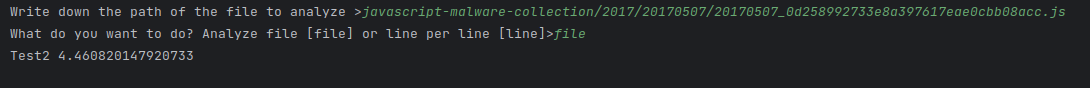
\includegraphics[width=18cm]{images/tool_1.png}
		\caption{Análisis del Fichero Completo}
	\end{figure}
	
	
	\begin{figure}[H]
		\centering
		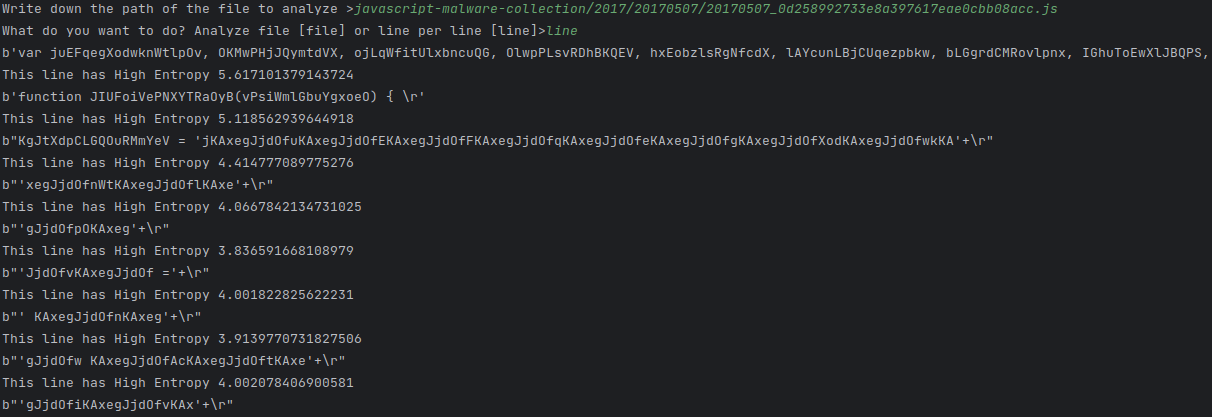
\includegraphics[width=18cm]{images/tool_2.png}
		\caption{Análisis del Fichero por Líneas }
	\end{figure}


	\newpage
	\section{Importancia de las amenazas de Javascript en Windows}
	Los ataques basados en script se han convertido en una amenaza importante en los últimos años. Algunas estimaciones sitúan estos ataques en el 40 por ciento o más de todos los ciber ataques globales. Un script pude ser cualquier cosa, desde una secuencia de comandos simples utilizados para la configuración del sistema, la automatización de  tareas y otros fines generales, hasta un código mucho más avanzado, de múltiples capas y ofuscado. Entre los lenguajes de scripting más utlizados se encuentran PowerShell, VBScript y JavaScript.
	
	Si bien los ataques de PowerShell son los más utilizados, los actores de amenazas maliciosos también utilizan JavaScript de Windows para muchos de los mismos fines. Fuera de un navegador, que ejecuta JavaScript de forma encapsulada, lo que limita en gran medida la interacción de ese código en el sistema operativo, Windows proporciona funciones para la ejecución de JavaScript con Windows Script Host (WSH), que ejecuta JavaScript (y otros lenguajes de secuencias de comandos compatibles con Windows) bajo los procesos de Windows \textit{wscript.exe} y \textit{cscript.exe}, lo que proporciona una superficie de ataque que los adversarios pueden aprovechar.
	
	El malware JavaScript puede variar desde un simple dropper destinado a entregar malware adicional hasta partes de malware multipropósito con todas las funciones.
	
	A continuación se enumerarán ejemplos de malware prominentes en el panorama JavaScript "puro" que a menudo desafían las firmas de detección estáticas mediante una gran ofuscación de código y sin emplear archivos binarios compilados. \cite{javascript_malware}
	
	\subsection{WJworm}
	\textit{Vengeance Justice Worm} es un malware en JavaScript que combina caracrerísticas de Gusano, Robo de Información, Troyano de Acceso Remoto (RAT), Malware de Denegación de Servicio (DOS) y spam-bot.Fue descubierto en 2016.
	
	Se propaga por adjuntos de email infectando dispositivos de almacenamiento externo.
	
	Una vez que se ejecuta por la víctima, el VJWorm ofuscado, enumera los dispositivos instalados, y si un dispositivo se encuentra, lo infecta.
	
	Obtiene información del sistema, del usuario, el anti-virus instalado, las cookies del navegador, la presencia de \textit{vbc.exe} en el sistema (Compilador de Microsoft .NET de Visual Basic) para comprobar si .NET está instalado en el sistema y puede afectar para instalar malware adicionar.
	
	VJWorm enviará la información al Servidor de Command-and-Control y esperará las siguientes instrucciones como descargar y ejecutar malware adicional.
	
	\subsection{WSHRat}
	
	También conocido como Houdini, H-worm, Dunihi y otros alias, es otro malware \textit{commodity malware} \footnote{RAT, Troyano de Acceso Remoto.}. Descubierto en 2013, fue desarrollado iriginalmente en VBS. Su variante en 2019, emergió en una versión de JavaScript de la versión inicial.
	
	Como todos los Troyanos de acceso remoto (RATs), el propósito principal de WSHRAT es mantener el acceso a la máquina, ejecutando comandos remotos y descargar malware adicional.
	
	Se propaga por adjuntos de email y también es capaz de infectar dispositivos externos.
	
	Una vez ejecutado por la víctima, el altamente ofuscado WSHRat seguirá un proceso similar al descrito anteriormente con VJworm, para obtener los datos del usuario y del sistema y reportarlos al Command-and-Control. A continuación infectar los dispositivos de almacenamiento externo y esperar a las siguientes instrucciones.
	
	Las variantes en VBS han sido reportadas recientemente, involucradas en campañas de espionaje en la industria aeronáutica.
	
	\subsection{STRRAT}
	Es un RAT basado en Java, con un dropper/wrapper en JavaScript que fue descubierto en 2020. Su payload core (fichero .jar) contiene varias capas de ofuscación y codificación dentro del JavaScript wrapper/dropper.
	
	STRRAT se propaga por adjuntos en emails. Su capacidad incluye funcionalidades de RAT (acceso remoto, ejecución remota de comandos), browser, email client harvesting \footnote{Conseguir cuentas de correo} y una funcionalidad ransomware, cifrando los ficheros añadiendo una extensión \textit{.crimson} al dispositivo, que pueden ser recuperados fácilmente si su contenido no se modifica.
	
	A diferencia de otros malware hechos en Java, no requiere tener Java instalado para infectar al sistema y funcionar. Cuando el dropper/wrapper de JavaScript se ejecute, se instala una versión de Java para que pueda ejecutarse el malware.	
	

	\subsection{BlackByte Ransomware}
	Es un Ransomware que ha sido recientemente descubierto con un core payload que es una .DLL desarrollada en .NET con un wrapper en JavaScript. Emplea una ofuscación muy alta tanto el wrapper como la .DLL.
	
	Una vez que el wrapper es ejecutado, el malware desofusca el payload lo ejecuta en memoria. La .DLL se descarga y BlackByte hará un checkeo del Sistema Operativo instalado y finaliza si el lenguaje del sistema es de Europa del Este.
	
	A continuación chequeará la presencia de antivirus y sandbox relacionados con .DLL, intentando bypasear la AMSI \footnote{Interfaz de examen antimalware}, borrar las shadow copies \footnote{Copias de Seguridad} del sistema para evitar la recuperación del sistema y modificar algunos servicios del sistema como el Firewall. Cuando el sistema esté preparado para encriptar los ficheros, descargará una clave simétrica que utilizará para encriptar los ficheros del sitema, si este fichero no lo encuentra, finaliza su ejecución.
	
	A diferencia de la mayoría del Ransonmware actual, BlackByte utilizar una clave de cifrado simétrica ni genera una clave única de cifrado para cada víctima, lo que quiere decir que la misma clave puede ser utilizada para desencriptar todos los ficheros que el malware ha encriptado.
	
	Esto facilita el manejo de las claves para los actores de BlackByte, a costa de un esquema de encriptación más débil y una recuperación del sistema más fácil.
	
	Como la mayoría de los Ransomware, tiene capacidad de gusano para infectar más puntos de la misma red.
	
	
	\subsection{Carbanak/FIN7 JavaScript Backdoor}
	Descubierto en 2014, son uno de los actores de amenazas con motivación financiera más prolíficos y exitosos en acción de la actualidad, responsables de pérdidas estimadas en mil millones de dólares para innumerables instituciones financieras en todo el mundo.
	
	El principal medio para difundir su malware consiste en correos electrónicos de Phishing dirigidos y eficaces.
	
	Sin embargo, se ha descubierto recientemente una backdoor en JavaScript asociada con el actor, parece indicar que su malware que estaba basado principalmente en PowerShell, ha sido migrado a JavaScript en un intento de volverse menos detectable para los proveedores de seguridad.
	
	Una vez ejecutada, la backdoor iniciará un delay de dos minutos en un esfuerzo por evitar la detección automatizada de la Sandbox y luego recabará la información de la máquina infectada: su IP, su MAC, el hostname de su DNS y lo reportará al servidor de Command-and-Control y ejecutará cualquier código que reciba como respuesta.
	
	Emplea Cobalt Strike\cite{cobaltstrike} como malware de seguimiento posterior a una infracción.\footnote{Herramienta de Red Team para probar los sitemas y sus mecanismos de protección. }
	
	\newpage
	\section{Pasos para Desofuscar un Código Malware en JavaScript\label{desobfuscation}}
		
	\subsection{JavaScript Beautifully}
	En ocasiones nos encontramos con código en JavaScript que está escrito en una sola línea, como ocurre con la muestra \textit{2b0c9059feece8475c71fbbde6cf4963132c274cf7ddebafbf2b0a59523c532e.js} del malware WJWorm. Para ello, tenemos que utilizar la herramienta JavSCript Beautify de \href{https://gchq.github.io/CyberChef}{CyberChef}
	
	\begin{figure}[H]
		\centering
		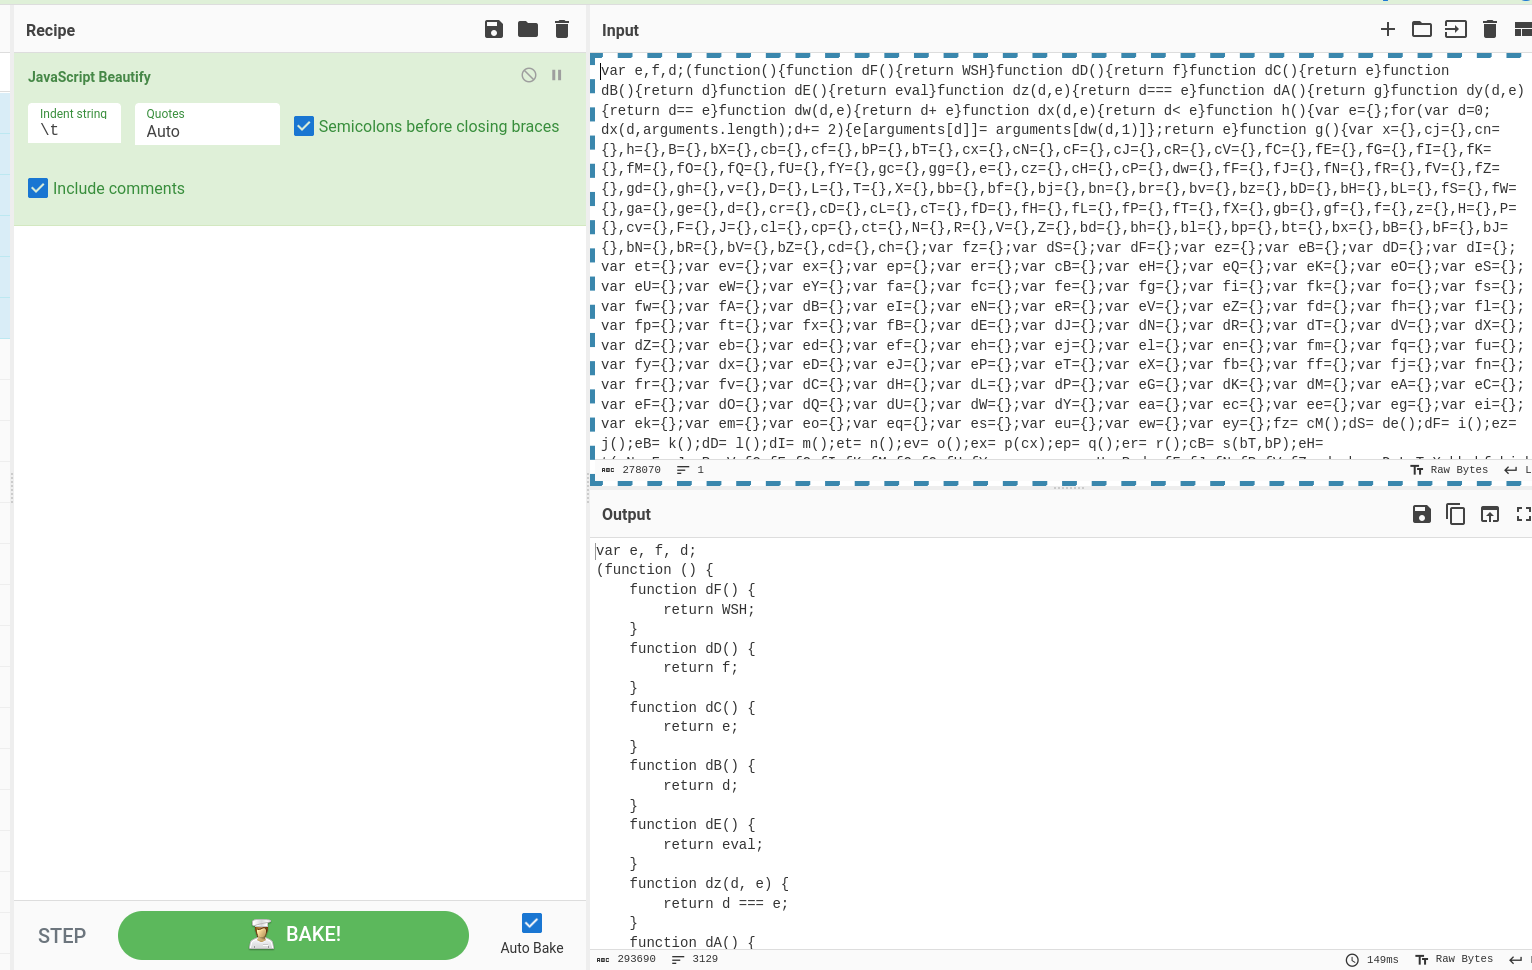
\includegraphics[width=18cm]{images/beautifully.png}
		\caption{CyberChef JavaScript Beautifully}
	\end{figure}
	
	\subsection{IIFE: Immediately Infoked Function Expression}
	Muestra \href{https://github.com/bl4de/research/blob/master/javascript-malware-obfuscation/do_not_run.js}{https://github.com/bl4de}
	
	Es una forma de ejecutar una función en JavaScript sin llamarla directamente.
	
	Considerando el siguiente ejemplo, no se va a ejecutar nada:
	\begin{scriptsize}
		\estiloR
		\begin{lstlisting}[caption={Ejemplo de IIFFE}, language={Java}]
			function hello(message) {
				console.log(message)
			}
		\end{lstlisting}
	\end{scriptsize}
	Sin embargo, si ejecutamos este otro, sí se nos ejecutará la función:
	\begin{scriptsize}
		\estiloR
		\begin{lstlisting}[caption={Ejemplo de IIFFE}, language={Java}]
			function hello(message) {
				console.log(message)
			}
			
			hello('This is test')
		\end{lstlisting}
	\end{scriptsize}
	
	Ahora vamos a hacer IIFFE de este código. También se ejecutará la función.
	\begin{scriptsize}
		\estiloR
		\begin{lstlisting}[caption={Ejemplo de IIFFE}, language={Java}]
			(function hello(message) {
				console.log(message)
			})('This is test')
		\end{lstlisting}
	\end{scriptsize}

	Esto es posible por dos motivos:
	\begin{itemize}
		\item Los paréntesis alrededor de una expresión de una función hace que la expresión sea válida y se ejecute.
		\item En el paréntesis \verb|('This is test')| ejecuta la función pasando ese texto como argumento. Técnicamente \verb|(fn(x){})(x)| es equivalente a \verb|(fn(x)| pero con su ejecución incluida.
	\end{itemize}
	
	Entonces, si un malware tiene el siguiente código:
	
	\begin{scriptsize}
		\estiloR
		\begin{lstlisting}[caption={Ejemplo de IIFFE}, language={Java}]
			(function(quhuvu6) {
				
				// ...
				
			}("41553a304f0b442551284206" + "672651014d1e1a60127" + ...
		\end{lstlisting}
	\end{scriptsize}

	Significa que se ejecuta la función automáticamente con ese largo ASCII como argumento.
	
	\subsection{Expresiones, operador coma, parseInt() y toString()}
	Muestra \href{https://github.com/bl4de/research/blob/master/javascript-malware-obfuscation/do_not_run.js}{https://github.com/bl4de}
	
	Vamos a ver la siguiente función \verb|cicuza()|:
	
	\begin{scriptsize}
		\estiloR
		\begin{lstlisting}[caption={Ejemplo de operadores}, language={Java}]
			function cicuza(syhri) {
				var fahomyfo = [];
				for (var segovmiw4 = parseInt((0).toString(36)) /*CN1b367Z19XZqi8XgI67*/ ; segovmiw4 < syhri["l" + ("F", "T", "H", "e") + "n" + ("G", "n", "O", "g") + (29).toString(36) + ("u", "X", "U", "p", "h")]; segovmiw4 += parseInt((2).toString(36))) {
					fahomyfo[("E", "w", "f", "F", "p") + ("G", "i", "L", "u") + "s" + "h"](parseInt(syhri["s" + "u" + "b" + "s" + ("M", "h", "M", "U", "f", "t") + ("M", "q", "r")](segovmiw4, (85, 19, 84, 9, 2)), parseInt((42).toString(0x24)) /*uShFAoMcgqPvcds6w2xD*/ ));
				}
				return fahomyfo;
			};
			
		\end{lstlisting}
	\end{scriptsize}
	
	Vamos a renombrar \verb*|fahomyfo| a un nombre con sentido para verlo mejor. En la función, se declara esta variable como array y luego tras un for y cierta lógica, se devuelve un resultado,a sí que llamaremos a la variable \verb*|result|:
	\begin{scriptsize}
		\estiloR
		\begin{lstlisting}[caption={Ejemplo de operadores}, language={Java}]
			function cicuza(syhri) {
				var result = [];
				for (var segovmiw4 = parseInt((0).toString(36)) /*CN1b367Z19XZqi8XgI67*/ ; segovmiw4 < syhri["l" + ("F", "T", "H", "e") + "n" + ("G", "n", "O", "g") + (29).toString(36) + ("u", "X", "U", "p", "h")]; segovmiw4 += parseInt((2).toString(36))) {
					result[("E", "w", "f", "F", "p") + ("G", "i", "L", "u") + "s" + "h"](parseInt(syhri["s" + "u" + "b" + "s" + ("M", "h", "M", "U", "f", "t") + ("M", "q", "r")](segovmiw4, (85, 19, 84, 9, 2)), parseInt((42).toString(0x24)) /*uShFAoMcgqPvcds6w2xD*/ ));
				}
				return result;
			};
			
		\end{lstlisting}
	\end{scriptsize}
		
	Ahora vamos a ver el bucle \verb*|for|. Primero definimos el valor inicial de la variable con la que empieza:
	\begin{scriptsize}
		\estiloR
		\begin{lstlisting}[caption={Ejemplo de operadores}, language={Java}]
			for (var segovmiw4 = parseInt((0).toString(36)) /*CN1b367Z19XZqi8XgI67*/ ; ....
		\end{lstlisting}
	\end{scriptsize}
	
	Con lo cual \verb*|parseInt((0).toString(36))| tiene dos operaciones concatenadas:
	
	\begin{itemize}
		\item \verb*|(0)| vale 0
		\item \verb*|.toString(36)| es un método que devuelve una representación de un objeto JavaScript. Cada objeto de JavaScript tiene este método, en este caso el número 0 será el 0 en representación de String.
		\item Cuando se llama a la función \verb*|.toString| con un número como parámetro, que puede ser un número entero entre 2 y 36 especificando la base en la que se representará el valor numérico. Así que en este caso será el número 0 en base 36. Resultando el número \verb*|0|
	\end{itemize}

	En la segunda llamada \verb*|parseInt(0)| devuelve 0 también. Este método parsea cualquier String a su valor Entero y si la conversión no es posible, devuelve un \verb*|NaN|, Not a Number. Entonces el resultado será \textbf{0}.
	
	Vamos a renombrar la variable \verb*|segovmiw4| como \verb*|i| y poner el 0 como inicial:
	
	\begin{scriptsize}
		\estiloR
		\begin{lstlisting}[caption={Ejemplo de operadores},language={Java}]
			function cicuza(syhri) {
				var result = [];
				for (var i = 0; i < syhri["l" + ("F", "T", "H", "e") + "n" + ("G", "n", "O", "g") + (29).toString(36) + ("u", "X", "U", "p", "h")]; i += parseInt((2).toString(36))) {
					result[("E", "w", "f", "F", "p") + ("G", "i", "L", "u") + "s" + "h"](parseInt(syhri["s" + "u" + "b" + "s" + ("M", "h", "M", "U", "f", "t") + ("M", "q", "r")](i, (85, 19, 84, 9, 2)), parseInt((42).toString(0x24)) /*uShFAoMcgqPvcds6w2xD*/ ));
				}
				return result;
			};
		\end{lstlisting}
	\end{scriptsize}
	Ahora nos vamos a enfocar en el siguiente código:
	\begin{scriptsize}
		\estiloR
		\begin{lstlisting}[caption={Ejemplo de operadores}, language={Java}]
			i < syhri["l" + ("F", "T", "H", "e") + "n" + ("G", "n", "O", "g") + (29).toString(36) + ("u", "X", "U", "p", "h")];
		\end{lstlisting}
	\end{scriptsize}
	
	Como sabemos, se puede leer un String como si fuese un array. Pero lo curioso es que en este caso se están utilizando paréntesis: \verb*|("F", "T", "H", "e")|. Si probamos a ejecutar \verb*|("F")| y \verb*|("F", "T", "H", "e")| vemos que las comas, lo que hace es separar los valores y sólo se utiliza el último valor:
	
	\begin{figure}[H]
		\centering
		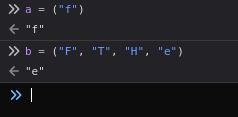
\includegraphics[width=6cm]{images/string.png}
		\caption{Conjunto de Caracteres String}
	\end{figure}
	
	Podemos leer los primeros caracteres dentro de \verb*|i < syhri[...]| que son \verb*|l e n g|, el quinto es una construcción como la anterior pero en este caso \verb*|(29).toString(36)| que es el la 29 cifra Hexadecimal que es la \verb*|t|. La última expresión devuelve la \verb*|h| y finalmente con la concatenación del operador \verb*|+| podemos ver que el resultado es \verb*|syhri["length"]|.
	
	Si renombramos esa variable como \verb*|val| y desofuscamos la última parte, podemos ver que \verb*|parseInt((2).toString(36))| es el número 2 en formato String.
	
	Entonces, hasta ahora tenemos lo siguiente:
	
	\begin{scriptsize}
		\estiloR
		\begin{lstlisting}[caption={Ejemplo de operadores}, language={Java}]
			function cicuza(val) {
				var result = [];
				for (var i = 0; i < val["length"]; i += 2) {
					result[("E", "w", "f", "F", "p") + ("G", "i", "L", "u") + "s" + "h"](parseInt(val["s" + "u" + "b" + "s" + ("M", "h", "M", "U", "f", "t") + ("M", "q", "r")](i, (85, 19, 84, 9, 2)), parseInt((42).toString(0x24)) /*uShFAoMcgqPvcds6w2xD*/ ));
				}
				return result;
			};
		\end{lstlisting}
	\end{scriptsize}
	
	Utilizando los métodos anteriores, podemos observar que el array quedará como \verb*|result["push"]|.
	
	JavaScript puede llamar cada Objeto utilizando el \verb*|.|. Por ejemplo si tenemos un array llamado \verb*|arr|, podemos llamar a su método \verb*|push| con el punto:
	
	\begin{scriptsize}
		\estiloR
		\begin{lstlisting}[caption={Ejemplo de operadores}, language={Java}]
			let arr = [] // declare Array object named arr
			arr.push(10) // adds 10 as a first element of Array arr
			arr.push(20) // adds 20 as a second element
			console.log(arr) // prints [10, 20]
		\end{lstlisting}
	\end{scriptsize}
	
	Si observamos la siguiente línea:
	\begin{scriptsize}
		\estiloR
		\begin{lstlisting}[caption={Ejemplo de operadores}, language={Java}]
			parseInt(val["s" + "u" + "b" + "s" + ("M", "h", "M", "U", "f", "t") + ("M", "q", "r")](i, (85, 19, 84, 9, 2)), parseInt((42).toString(0x24)) /*uShFAoMcgqPvcds6w2xD*/ )
		\end{lstlisting}
	\end{scriptsize}

	Devolverá la función \verb*|substr| que tiene dos argumentos, el primero es el índice del primer char de la parte a devolver y el segundo (opcional) es el tamaño, sino, se parte hasta el final del String.
	
	Así que tendremos lo siguiente hasta ahora:
	\begin{scriptsize}
		\estiloR
		\begin{lstlisting}[caption={Ejemplo de operadores}, language={Java}]
			parseInt(val["substr"](i, (85, 19, 84, 9, 2)), parseInt((42).toString(0x24)) /*uShFAoMcgqPvcds6w2xD*/ )
		\end{lstlisting}
	\end{scriptsize}

	

	\begin{scriptsize}
		\estiloR
		\begin{lstlisting}[caption={Ejemplo de operadore}, language={Java}]
			val["substr"](i, 2)
		\end{lstlisting}
	\end{scriptsize}
	
	 La última parte, \verb*|parseInt((42).toString(0x24))| que como sabemos parsea 42 a un entero utilizando la base \verb*|0x24|, que al ser un valor Hexadecimal, su valor decimal será 36. Convirtiendo a String este valor, tendremos el valor 16.
	
	\begin{scriptsize}
		\estiloR
		\begin{lstlisting}[caption={Ejemplo de operadores desofuscado}, language={Java}]
			function cicuza(val) {
				var result = [];
				for (var i = 0; i < val.length; i += 2) {
					result.push(parseInt(val.substr(i, 2), 16));
				}
				return result;
			};
		\end{lstlisting}
	\end{scriptsize}
	
	Lo que hace esta función es que el argumento \verb*|val| tiene como valor inicial un String extremadamente largo, la función itera sobre el mismo, sustrae cada 2 caracteres, los convierte de Hexadecimal a Decimal y finalmente lo devuelve como un array.
	
	Si cogemos la primera parte del String \verb*|"41553a304f0b442551284206"|, 41 pasa a ser 65, 55, 85, 3a se convierte en 58, 30 en 48, 4f en 79 y así en adelante. Al final acabará siendo un array que contiene valores decimales, que será la variable \verb*|defiq| del malware
	\begin{scriptsize}
		\estiloR
		\begin{lstlisting}[caption={Ejemplo de operadores final}, language={Java}]
			(...)
			var defiq = cicuza(quhuvu6);   // here we are so far :)
			var permy = "H@D~7a84O";
			var paghimqycgi = {
				getpy: "myqniroqa3"
			};
			
			(...)
		\end{lstlisting}
	\end{scriptsize}

	\subsection{Consiguiendo el constructor de la función}
	Un método muy utilizado en la ofuscación de malware en JavaScript , es ocultar las definiciones de funciones y sus llamadas. Por ejemplo:
	
	\begin{scriptsize}
		\estiloR
		\begin{lstlisting}[caption={Ejemplo ofuscación con constructor}, language={Java}]
			function doubleX(x) {
				return x * 2
			}
			
			doubleX(10) // returns 20
		\end{lstlisting}
	\end{scriptsize}

	Vamos a ofuscar este código:
	\begin{scriptsize}
		\estiloR
		\begin{lstlisting}[caption={Ejemplo ofuscación con constructor}, language={Java}]
			let xcf = new Function("x","return x * 2")
			
			xcf(10)   // returns 20 as well
		\end{lstlisting}
	\end{scriptsize}

	\verb*|Function| es un método en JavaScript que construye una nueva función, como argumentos acepta una lista que es lo que tiene que devolver y el último argumento, el cuerpo de la función.
	
	Sin embargo, el método \verb*|a.forEach| tiene su propia propiedad llamada \verb*|constructor| que que es \verb*|Function()| ella misma.
	
	Es decir, sustituyendo el código anterior:
	\begin{scriptsize}
		\estiloR
		\begin{lstlisting}[caption={Ejemplo ofuscación con constructor}, language={Java}]
			let xcf = a.forEach.constructor("x","return x * 2")
			
			xcf(10)  // yep, it works! 20
		\end{lstlisting}
	\end{scriptsize}
	
	Hay un método muy similar en el código de nuestro malware:
		
	\begin{scriptsize}
		\estiloR
		\begin{lstlisting}[caption={Ejemplo ofuscación con constructor}, language={Java}]
			let sdfgfdg = "".substr
			sdfgfdg.call("malware",1,2)   // "al"
		\end{lstlisting}
	\end{scriptsize}

	Este código equivale a:

	\begin{scriptsize}
		\estiloR
		\begin{lstlisting}[caption={Ejemplo ofuscación con constructor}, language={Java}]
			"malware".substr(1,2)  // "al"
		\end{lstlisting}
	\end{scriptsize}

	Esto pasa con los métodos \verb*|call()|, \verb*|apply()| y con \verb*|bind()| también.
	
	Vamos a aplicar esto al código de nuestro malware:
	\begin{scriptsize}
		\estiloR
		\begin{lstlisting}[caption={Ejemplo ofuscación con constructor}, language={Java}]
			var xewubdiwhit = "kydka"[(12).toString(36) + (24).toString(36) + ("r", "w", "h", "Z", "n") + ("n", "X", "L", "s", "w", "s") + "t" + (27).toString(36) + "u" + "c" + ("d", "m", "b", "t") + ("z", "E", "z", "n", "o") + ("N", "J", "r")];
		\end{lstlisting}
	\end{scriptsize}
	
	Entonces esto acabará siendo:
	\begin{scriptsize}
		\estiloR
		\begin{lstlisting}[caption={Ejemplo ofuscación con constructor}, language={Java}]
			var xewubdiwhit = "kydka"["constructor"]
		\end{lstlisting}
	\end{scriptsize}
	
	Que es lo mismo que:
	
	\begin{scriptsize}
		\estiloR
		\begin{lstlisting}[caption={Ejemplo ofuscación con constructor}, language={Java}]
			var fnConstructor = String.constructor
		\end{lstlisting}
	\end{scriptsize}
	Así que el código de nuestro malware quedará de la siguiente manera:
	\begin{scriptsize}
		\estiloR
		\begin{lstlisting}[caption={Ejemplo ofuscación con constructor}, language={Java}]
			(function(quhuvu6) {
				var defiq = cicuza(quhuvu6);
				var permy = "H@D~7a84O";
				var paghimqycgi = {
					getpy: "myqniroqa3"
				};
				var fnConstructor = String.constructor;
				var tyttaluli = "mokzine";
				
				var dikol = [];
				var mirjokbynet = 1;  // (27, 50, 52, 21, 1) equals 1
				
				(...)
		\end{lstlisting}
	\end{scriptsize}
	
	\subsection{Operadores Lógicos}
	Si analizamos el siguiente fragmento:
	
	\begin{scriptsize}
	\estiloR
	\begin{lstlisting}[caption={Ejemplo de Operadores Lógicos},  language={Java}]
   while (mirjokbynet <= permy[("h", "g", "B", "W", "l") + "e" + (23).toString(0x24) + "g" + ("u", "Z", "W", "u", "t") + (17).toString(36)]) {
			dikol = (permy[("M", "H", "s") + ("C", "N", "D", "u") + (11).toString(0x24) + (28).toString(0x24) + ("T", "k", "t") + "r"](permy[(21).toString(0x24) + "e" + "n" + (16).toString(36) + ("L", "S", "x", "t") + ("I", "D", "h") /*Q5E278CBpoixvOtUNpix*/ ] - mirjokbynet))[("d", "R", "p", "s") + ("H", "K", "A", "s", "D", "p") + "l" + "i" + ("Y", "b", "h", "t") /*O7MOfVrRkP9RlXlfKLxi*/ ]('');
			for (var juqno = +!!false; juqno < defiq[("R", "t", "E", "l") + ("y", "e", "f", "R", "e") + (23).toString(36) + (16).toString(36) + "t" + "h" /*H3RMPYzEeu55OVeGgb1v*/ ]; juqno++) {
				defiq[juqno] = defiq[juqno] ^ dikol[juqno % dikol["l" + (14).toString(36) + "n" + (16).toString(0x24) + (29).toString(0x24) + ("X", "O", "c", "m", "h")]]["c" + ("G", "w", "R", "e", "h") + (10).toString(36) + ("A", "W", "V", "i", "r") + "C" + ("Z", "O", "W", "o") + ("R", "N", "A", "y", "d") + "e" + "A" + "t" /*YZz3OuivKuwgqjkFVKu0*/ ]((88, 53, 3, 90, 0));
			}
			mirjokbynet++;
		};
		\end{lstlisting}
	\end{scriptsize}

	Además de lo que hemos visto anteriormente, hay unos usos extraños a la hora de utilizar operadores lógicos.
	
	Primero, vamos a simplificar el código y desofuscarlo con las técnicas que ya conocemos, además de renombrar \verb*|mirjokbynet| a \verb*|k| yu \verb*|juqno| a \verb*|j| también:
	
	\begin{scriptsize}
		\estiloR
		\begin{lstlisting}[caption={Ejemplo de Operadores Lógicos}, language={Java}]
			
			while (k <= permy.length) {
				dikol = (permy.substr(permy.length - k)).split('');
				for (var j = +!!false; j < defiq.length; j++) {
					defiq[j] = defiq[j] ^ dikol[j % dikol.length].charCodeAt(0);
				}
				k++;
			};
		\end{lstlisting}
	\end{scriptsize}
	
	Si observamos la variable de la condición del \verb*|while| llamada \verb*|permy| se utiliza y su definición asigna \verb*|"H@D~7a84O| al principio del script \verb*|var permy = "H@D~7a84O";|
	
	Ahora analizaremos el fragmento:
	
	\begin{scriptsize}
		\estiloR
		\begin{lstlisting}[caption={Ejemplo de Operadores Lógicos}, language={Java}]
		 while (k <= 9) {   // 9 is value of permy.length
		\end{lstlisting}
	\end{scriptsize}

	La siguiente línea, define el valor de \verb*|dikol|:
	
	\begin{scriptsize}
		\estiloR
		\begin{lstlisting}[caption={Ejemplo de Operadores Lógicos}, language={Java}]
			dikol = (permy.substr(permy.length - k)).split('');
		\end{lstlisting}
	\end{scriptsize}
	
	Como en este caso \verb*|k| es 0, \verb*|dikol| va a ser el último elemento del string \verb*|permy| que se parte en un array con la orden \verb*|split('')|, así que su valor en la primera iteración del while es \verb*|[0]|.
	
	Ahora vamos a la parte del for:
	
	\begin{scriptsize}
		\estiloR
		\begin{lstlisting}[caption={Ejemplo de Operadores Lógicos}, language={Java}]
			for (var j = +!!false; j < defiq.length; j++) {
				defiq[j] = defiq[j] ^ dikol[j % dikol.length].charCodeAt(0);
			}
		\end{lstlisting}
	\end{scriptsize}
	
	¿Qué evalua \verb*|+!!false|?
	\begin{itemize}
		\item inicialmente es \verb*|false|
		\item luego, el primer \verb*|!| que es un NOT lógico, lo cambia a \verb*|true|
		\item más tarde, el siguiente \verb*|!| lo vuelve a cambiar a \verb*|false|
		\item finalmente, el \verb*|+| hace un casting de Booleano a Entero, de \verb*|false| al valor \verb*|0|
	\end{itemize}
	
	\begin{figure}[H]
		\centering
		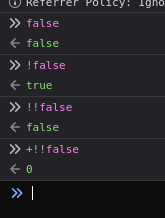
\includegraphics[width=5cm]{images/operators.png}
		\caption{Operadores lógicos}
	\end{figure}

	También tenemos otros operadores lógicos dentro del bucle for. Si nos fijamos \verb*|defiq| es un array con valores decimales (basándonos en las técnicas descritas anteriormente). Su primer elemento es el \verb*|65|. El resultado de la expresión \verb*|efiq[j] ^ dikol[j % dikol.length].charCodeAt(0)| se calcula de la siguiente manera:
	
	\begin{itemize}
		\item \verb*|j| es el valor de control del bucle. Comienza con el valor \verb*|0| así que el resultado \verb*|j % dikol.length| es \verb*|0| \verb*|(0 % 1 = 0)|. Recordemos que en esta iteración, \verb*|dikol.lenght| vale 1.
		\item ahora, tenemos la expresión \verb*|efiq[j] ^ dikol[0].charCodeAt(0)| que equivale a \verb*|65 ^ 79|. El primer elemento del array es 65 como resultado de \verb*|dikol[0].charCodeAt(0)| \verb*|dikol[0]| que es la \verb*|O| mayúscula. \verb*|'O'.charCodeAt(0)| es el número 79.
		\item el operador \verb*|^| es el operador XOR. El resultado de \verb*|65 ^ 79| es 14.
	\end{itemize}
	A continuación el bucle va a ir incrementando el valor de la variable k, comenzando la operación otra vez y el array con diferentes valores.
	
	
	\subsection{Ofuscación de caracteres y Strings}
	\subsubsection{Conjunto de enteros evaluados con eval}
	Nos podemos encontrar como en esta muestra, sacada de un pdf con \href{ [pdfstreamdumper](http://sandsprite.com/blogs/index.php?uid=7&pid=57)}{PDFStreamDumper}, un código JavaScript dentro de un documento PDF. Si nos fijamos, la función \verb*|var n = ""; eval(eval('Stri'+ n + 'ng.fr' + n + 'omCharC' + n + 'ode| con un listado de números. Si nos vamos a CyberChef, reemplazamos las comas por espacios y ejecutamos \textit{From Charcode} con la base en 10, vemos que se transforma en un código en Javascript. Este ejemplo está sacado de la Sample2.zip, la password es \textit{infected}:
	\begin{figure}[H]
		\centering
		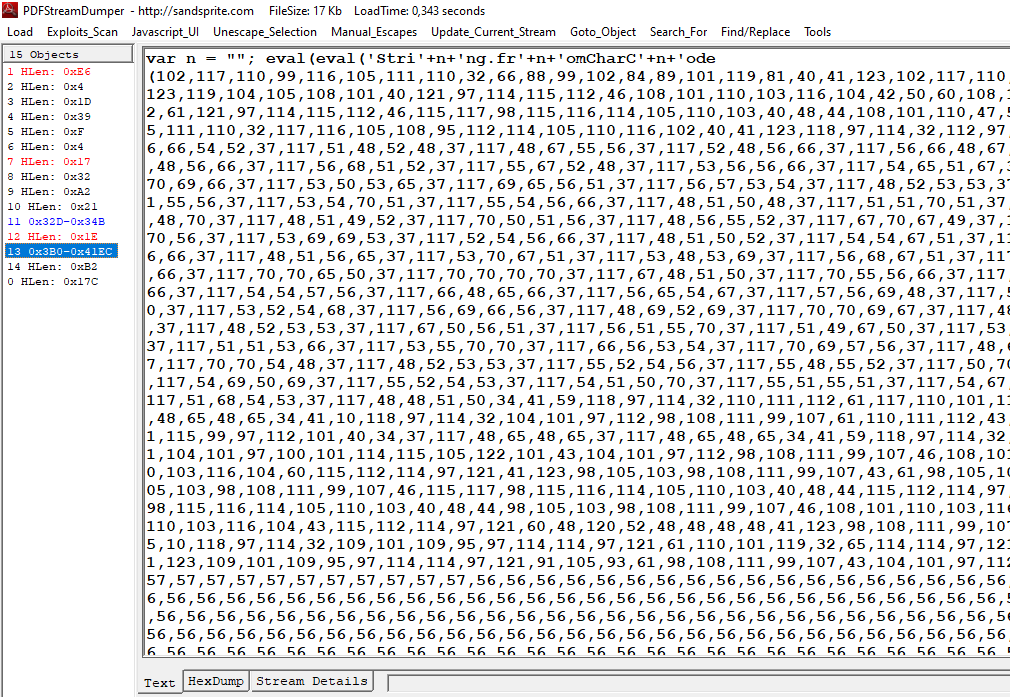
\includegraphics[width=18cm]{images/pdf1.png}
		\caption{Eval + conjunto de enteros}
	\end{figure}
	\begin{figure}[H]
		\centering
		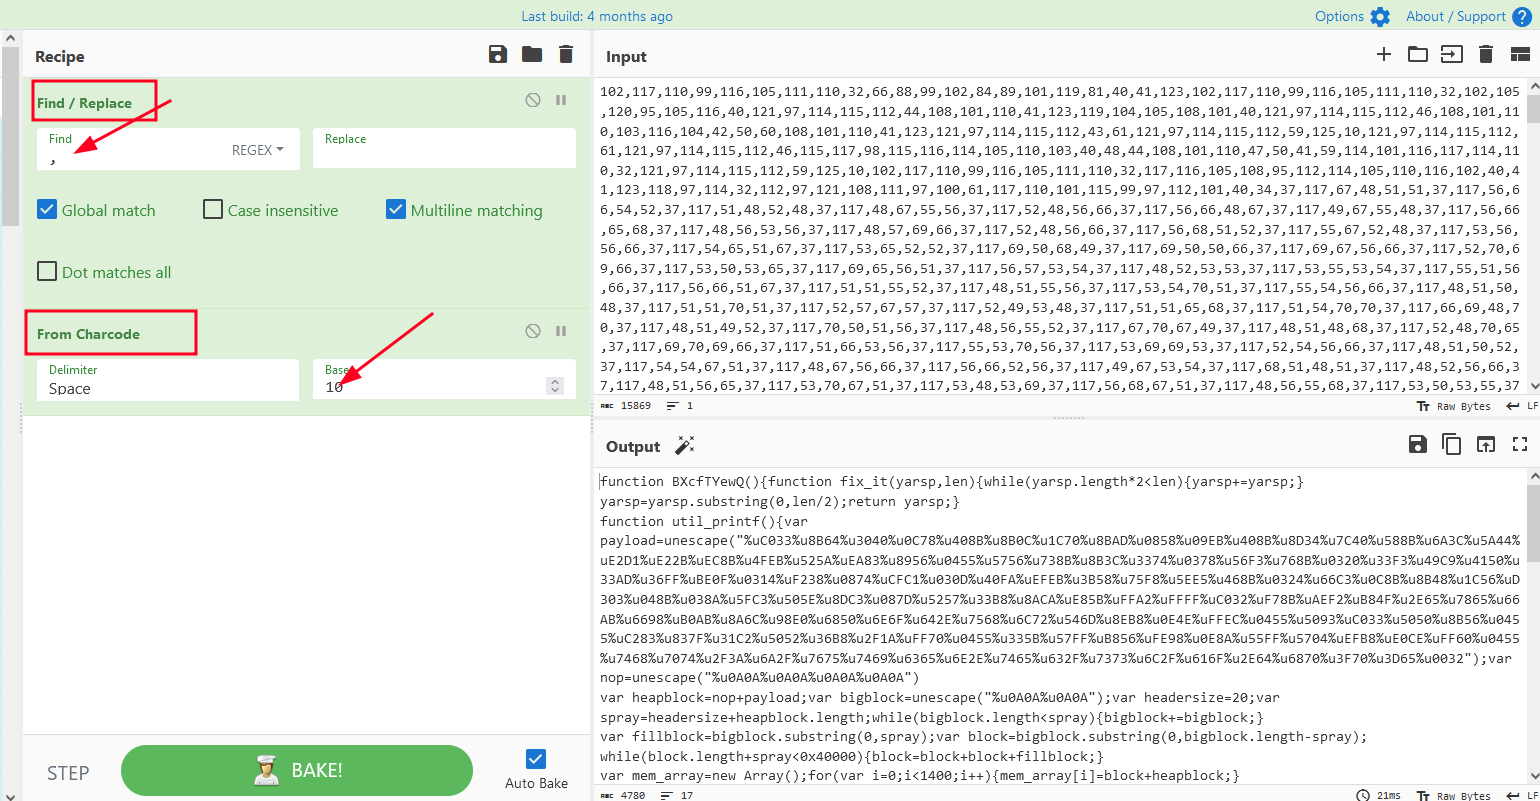
\includegraphics[width=15cm]{images/pdf2.png}
		\caption{Eval + conjunto de enteros}
	\end{figure}

	\subsubsection{Caracteres en Unicode}
	Podemos encontrarnos los caracteres en formato unicode, pero con la herramienta \textit{JavaScript Beautify} ya lo traduce automáticamente a la vez que formatea el código JavaScript:
	
	\begin{figure}[H]
		\centering
		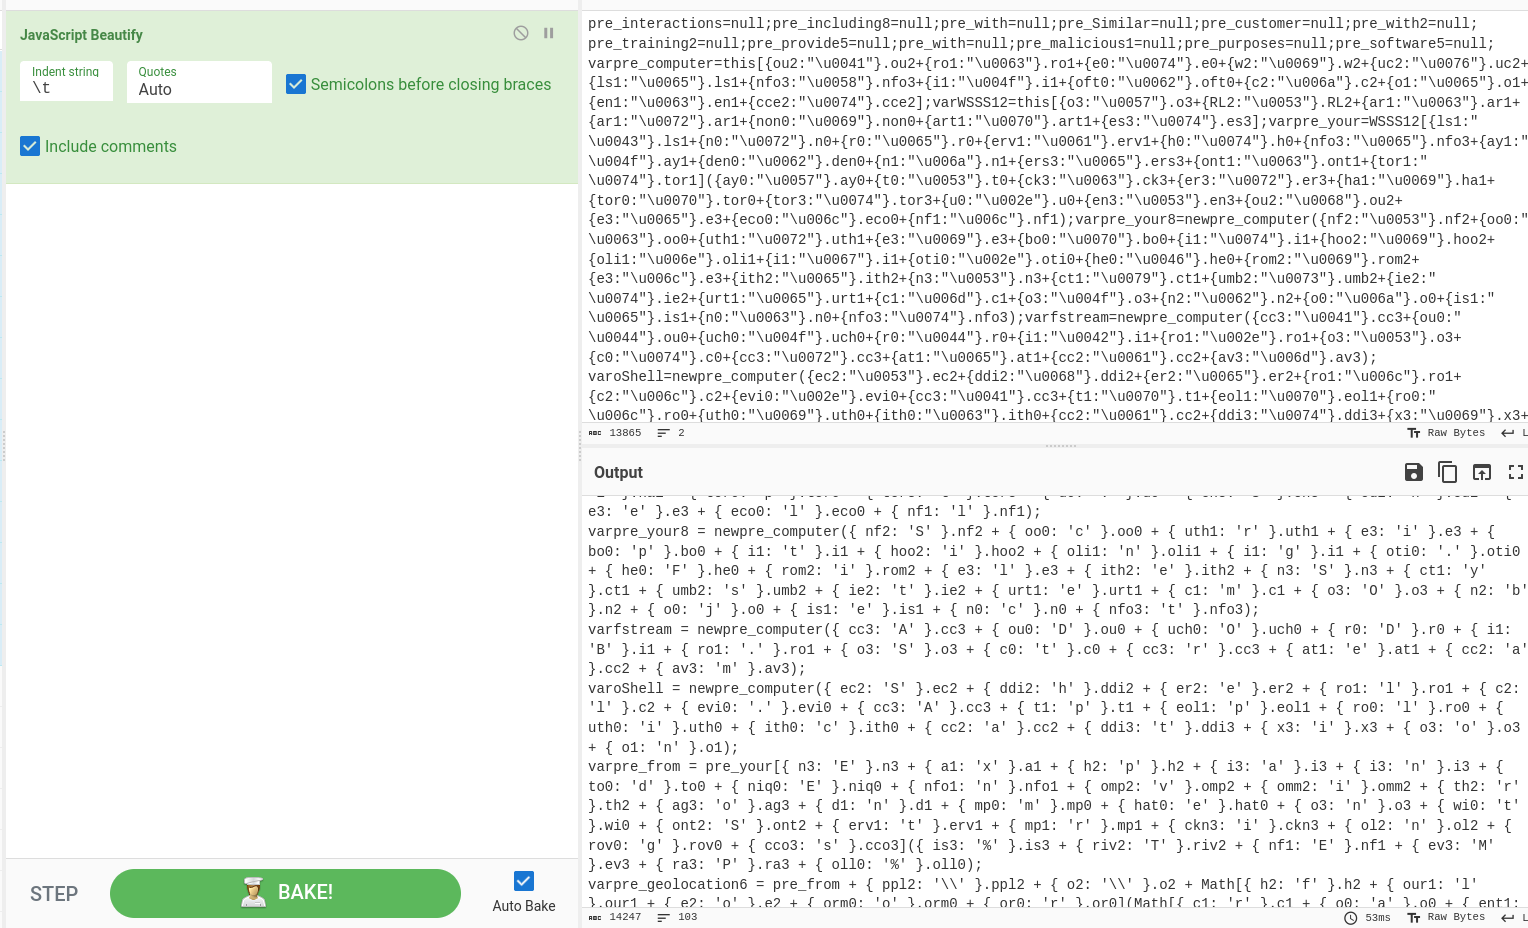
\includegraphics[width=15cm]{images/unicode.png}
		\caption{Caracteres unicode}
	\end{figure}

	\subsubsection{Caracteres en Hexadecimal}
	En el siguiente snippet del malware WSHRat \cite{javascript_malware}, podemos observar que tiene muchas partes que están ofuscadas en valores hexadecimales:
	\begin{figure}[H]
		\centering
		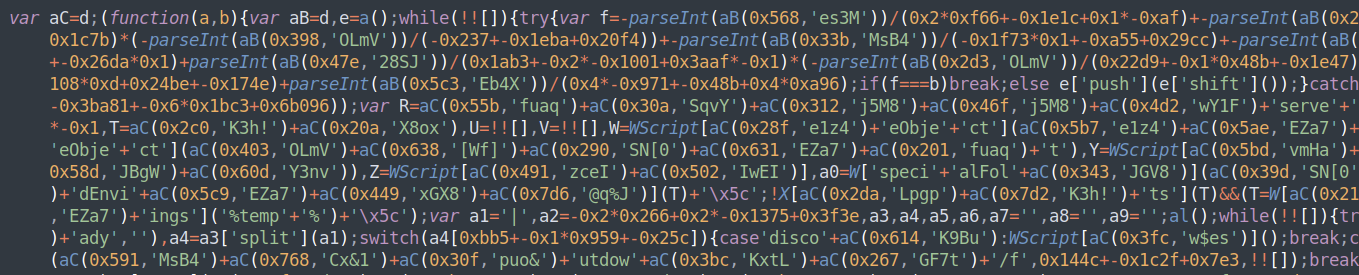
\includegraphics[width=15cm]{images/hexadecimal.png}
		\caption{Caracteres hexadecimales}
	\end{figure}

	\subsubsection{Caracteres de URL}
	El siguiente snippet de código de la versión de VB de STRRAT, como podemos observar, es una larga cadena de caracteres codificados en formato URL:
	\begin{figure}[H]
		\centering
		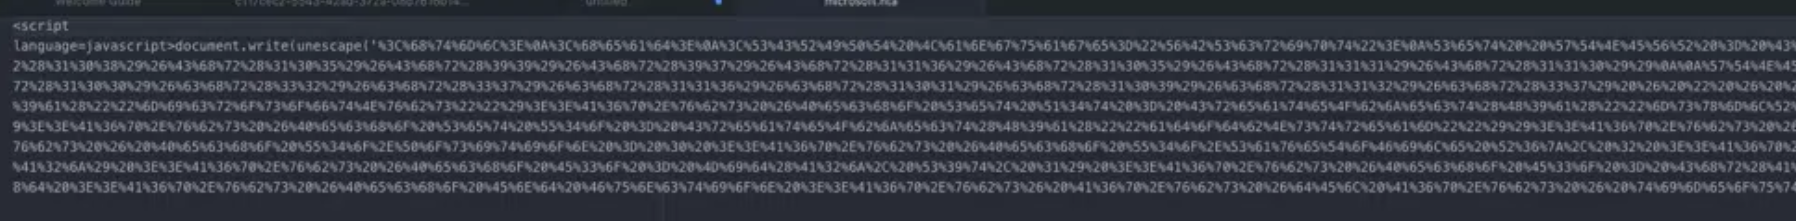
\includegraphics[width=18cm]{images/url_char.png}
		\caption{Caracteres hexadecimales}
	\end{figure}


	\subsection{Base64}
	El siguiente snippet de código forma parte del payload de STRRAT\cite{javascript_malware}, como podemos observar, es un largo Base64, que a continuación decodificará.
	
	\begin{figure}[H]
		\centering
		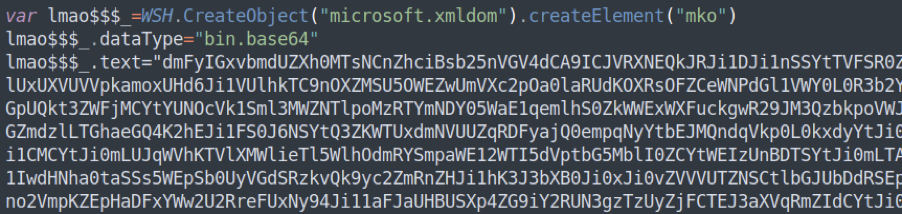
\includegraphics[width=15cm]{images/base64.png}
		\caption{Caracteres en base64}
	\end{figure}
	
	
	\newpage
	\section{Freyja Deobfuscation Tool}
	\href{https://github.com/drkrysSrng/freyja}{@drkrysSrng/freyja}
	
	Se ha desarrollado una herramienta, basándonos en los análisis que hemos mencionado anteriormente para facilitar la desofuscación de malware en JavaScript y su análisis. Tiene las siguientes funcionalidades:
	
	\begin{itemize}
		\item Limpia el código y lo tabula de manera similar, no sólo tabulando las instrucciones, sino que parsea los caracteres en hexadecimal y unicode.
		\item Chequeeo de la entropía con el algoritmo de Shannon, línea por línea o por texto completo.
		\item Cuando los caracteres Unicode o en Hexadecimal no están parseados ya que no están en formato String sino que es una variable ofuscada, se parsean a mayores también.
		\item Desofusca funciones como:
		\begin{itemize}
			\item \verb*|toString|, parsea los números a la base indicada y luego los pasa a string
			\item conjuntos de números dentro de \verb*|eval| a string
			\item evalúa y sustituye la función \verb*|unescape|
			\item evalúa la función \verb*|parseInt|
		\end{itemize}
		\item Concatena cadenas de caracteres separadas con el símbolo \verb*|+|
		\item Búsqueda de strings en base64 y su decodificación.
	\end{itemize}
	
	\subsection{Funcionamiento}
	Cuando ejecutamos al inicio la herramienta tenemos las siguientes opciones:
	\begin{figure}[H]
		\centering
		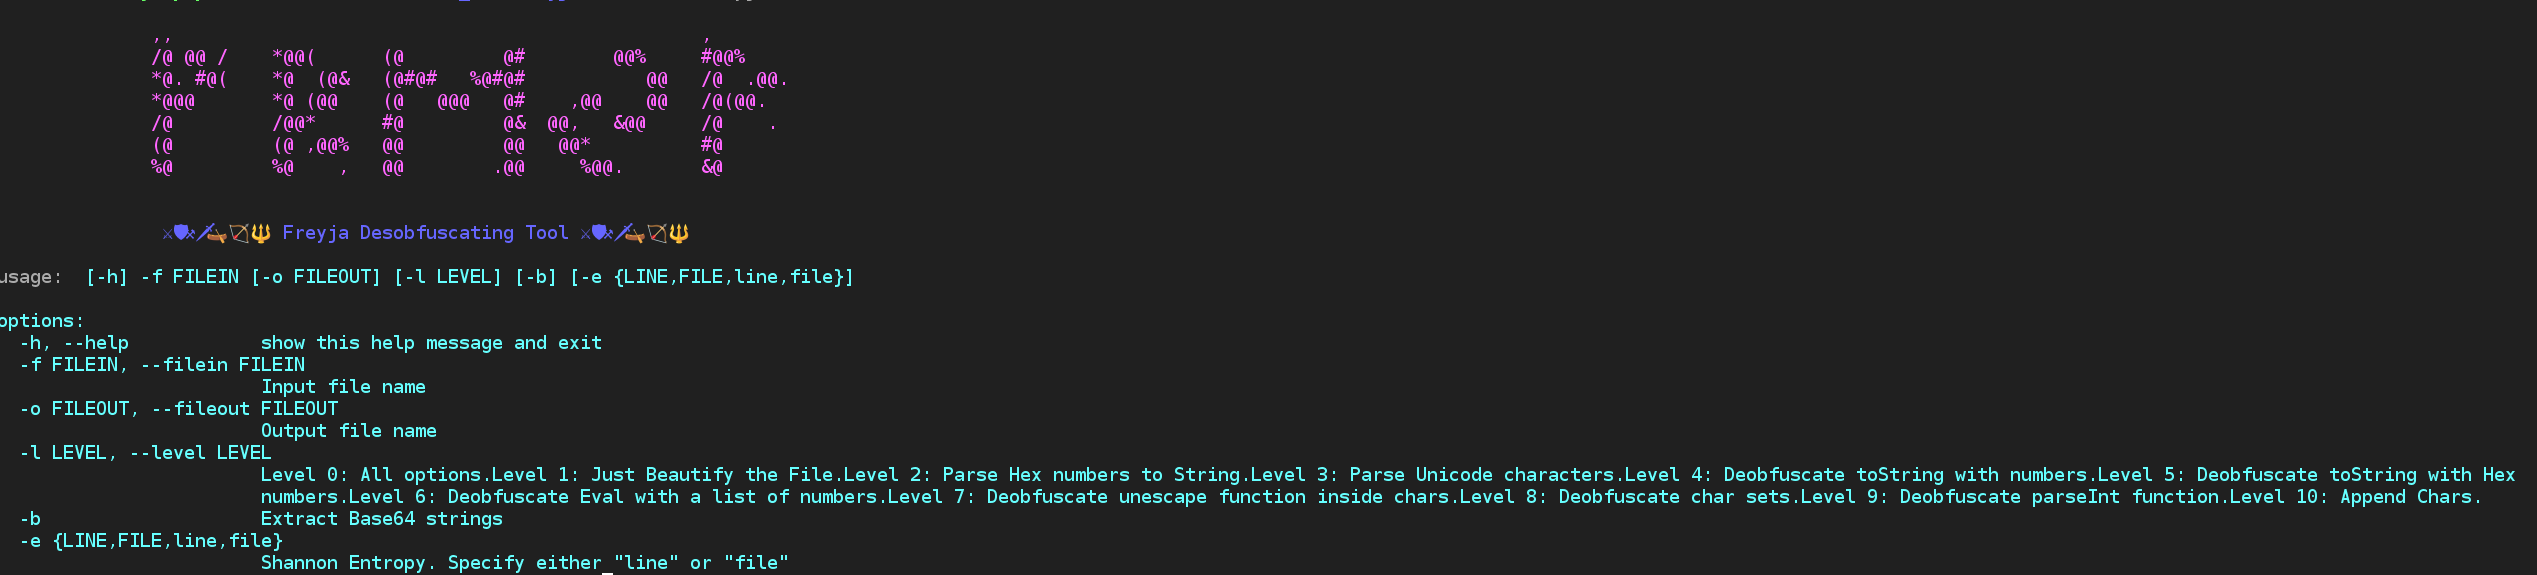
\includegraphics[width=18cm]{images/usage.png}
		\caption{Opciones de Freyja}
	\end{figure}
	
	\subsection{Entropía}
	Si queremos analizar la entropía de Shannon de un fichero, tenemos dos opciones: línea por línea o del fichero completo.
	La diferencia es que si lo hacemos línea por línea, solamente nos mostrará las líneas sospechosas ya que en teoría si la entropía nos da mayor de 3.75, se supone que ese texto no está escrito por un humano.
	
	\subsubsection{Línea por Línea}
	El comando sería:
		
	\begin{scriptsize}
		\estiloR
		\begin{lstlisting}[caption={Análisis de Entropía por líneas}, language={bash}]
			python freyja.py -f filein.js -e line
		\end{lstlisting}
	\end{scriptsize}
		
	\begin{figure}[H]
		\centering
		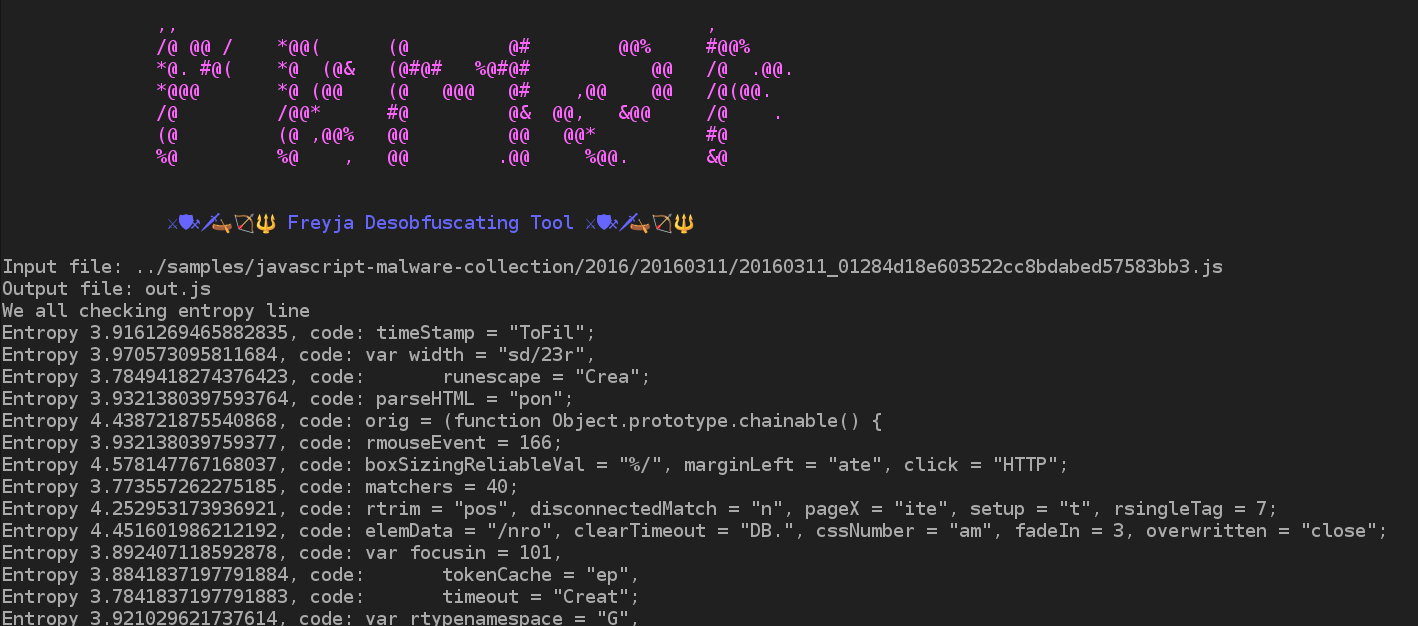
\includegraphics[width=18cm]{images/line_entropy.png}
		\caption{Entropía por líneas}
	\end{figure}
	\subsubsection{Fichero completo}
		El comando sería:
		\begin{scriptsize}
			\estiloR
			\begin{lstlisting}[caption={Análisis de Entropía del fichero completo}, language={bash}]
				python freyja.py -f filein.js -e file
			\end{lstlisting}
		\end{scriptsize}
				
				
		\begin{figure}[H]
			\centering
			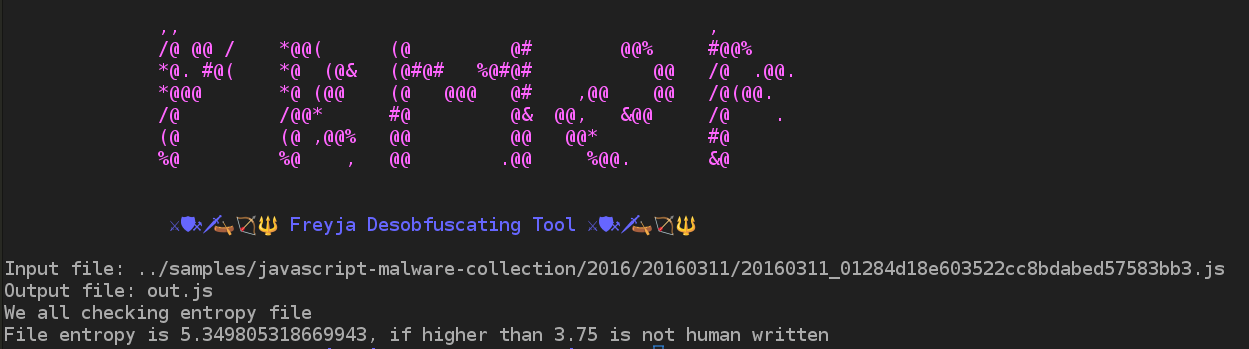
\includegraphics[width=18cm]{images/file_entropy.png}
			\caption{Entropía del fichero completo}
		\end{figure}
	
	\subsubsection{Código fuente}
	Similar al que se ha explicado en la sección \ref{entropy}, pero adaptado a nuestra tool:
	\begin{scriptsize}
		\estiloR
		\begin{lstlisting}[caption={Análisis de Entropía del fichero completo}, language={python}]
			
			"""
			    Calculates the Shannon entropy of a UTF-8 encoded string
			"""
			def entropy_check(string):
			    # decode the string as UTF-8
			    unicode_string = string.decode('utf-8')
			
			    # get probability of chars in string
			    prob = [float(unicode_string.count(c)) / len(unicode_string) for c in dict.fromkeys(list(unicode_string))]
			
			    # calculate the entropy
			    entropy = - sum([p * math.log(p) / math.log(2.0) for p in prob])
			
			    return entropy
			
			
			"""
			    Gets the string we are going to analyse, line per line or the full string from the file
			"""
			def calculate_entropy(filename, option):
			    option = option.upper()
			
			    if option == "FILE":
			        with open(filename, 'rb') as f:
			            content = f.read()
			            print(f"File entropy is {entropy_check(content)}, if higher than 3.75 is not human written")
			
			
			    elif option == "LINE":
			        with open(filename, 'rb') as f:
			            content = f.readlines()
			
			            for line in content:
			                entropy = entropy_check(line)
			                if entropy > 3.75:
			                    line_str = line[:-1]
			                    line_str = line_str.decode('utf-8')
			
			                    print(f"Entropy {entropy}, code: {line_str}")
			
			
		\end{lstlisting}
	\end{scriptsize}
	
	\subsection{Desofuscación}
	Se han desarrollado varias de las técnicas del apartado \ref{desobfuscation} en esta herramienta.
	Para que nos analice la herramienta el comando es el siguiente:
	\begin{scriptsize}
		\estiloR
		\begin{lstlisting}[caption={Desofuscación de ficheros JavaScript}, language={bash}]
			python freyja.py -f ./samples/simple_js_malware_code/do_not_run.js -o output.js -l 2
		\end{lstlisting}
	\end{scriptsize}
	\begin{itemize}
		\item \verb*|-f| Fichero a desofuscar.
		\item \verb*|-o| Fichero de salida desofuscado.
		\item \verb*|-l| Nivel de ofuscación. Le indicamos la técnica que queremos que utilice.
		\begin{itemize}
			\item Nivel 0: Todas las opciones
			\item Nivel 1: Técnica \textit{beautify}, tabular el fichero y darle formato al JavaScript.
			\item Nivel 2: Parsear los caracteres Hexadecimal a Strings.
			\item Nivel 3: Parsear los caracteres Unicode a Strings.
			\item Nivel 4: Desofuscar la función \verb*|toString|.
			\item Nivel 5: Desofuscar la función  \verb*|toString| con número hexadecimal.
			\item Nivel 6: Desofuscar la función  \verb*|eval| cuando tiene una lista de números.
			\item Nivel 7: Desofuscar la función  \verb*|unescape| cuando contiene caracteres.
			\item Nivel 8: Desofuscar conjuntos de caracteres.
			\item Nivel 9: Desofuscar la función  \verb*|parseInt|.
			\item Nivel 10: Concatena caracteres aunque estén en varias líneas.
		\end{itemize}
	\end{itemize}

	\subsubsection{Ejemplo de Nivel 1: Beautify}
	Para ello, se ha utilizado la librería \verb*|jsbeautifier| de Python:
	\begin{scriptsize}
		\estiloR
		\begin{lstlisting}[caption={Desofuscación de ficheros JavaScript Nivel 1: Beautify}, language={python}]
		"""
   Cleans the javascript file beautifying it
		"""
		def beautify_file(filename):
   res = jsbeautifier.beautify_file(filename, options)
		
   return res
		\end{lstlisting}
	\end{scriptsize}
	
	\begin{scriptsize}
		\estiloR
		\begin{lstlisting}[caption={Desofuscación de ficheros JavaScript Nivel 1: Beautify}, language={bash}]
			python freyja.py -f ./samples/Sample1/ejercicio6.js -l 1
		\end{lstlisting}
	\end{scriptsize}
	
	\begin{figure}[H]
		\centering
		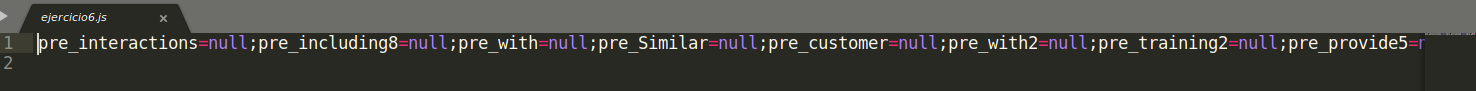
\includegraphics[width=18cm]{images/level1.png}
		\caption{Nivel 1: Beautify Ofuscado} 
	\end{figure}
	\begin{figure}[H]
		\centering
		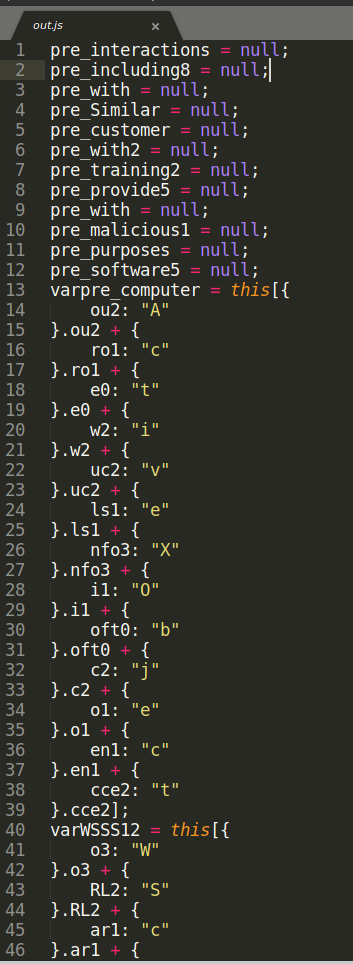
\includegraphics[width=5cm]{images/level1_after.png}
		\caption{Nivel 1: Beautify Desofuscado}
	\end{figure}
	
		\subsubsection{Ejemplo de Nivel 2: Parsear Hexadecimal}
		Para ello, se ha utilizado la librería \verb*|re| de Python, muy famosa para utilzar expresiones regulares. Se buscan los caracteres Hexadecimales que suelen ser 2 números que empiezan por \verb*|\x| y luego se parsean a String:
		\begin{scriptsize}
			\estiloR
			\begin{lstlisting}[caption={Desofuscación de ficheros JavaScript Nivel 2: Hexadecimal}, language={python}]

			"""
			    Parse hex numbers to char
			"""
			def parse_hex(data):
			    def replace_hex(match):
			        try:
			            decoded = bytes.fromhex(match.group(1)).decode('utf-8')
			        except UnicodeDecodeError:
			            decoded = bytes.fromhex(match.group(1)).decode("iso-8859-1")
			        return decoded
			
			    pattern = r'\\x([0-9a-fA-F]{2})'
			
			    data = re.sub(pattern, replace_hex, data)
			
			    return data
			\end{lstlisting}
		\end{scriptsize}
		
		\begin{scriptsize}
			\estiloR
			\begin{lstlisting}[caption={Desofuscación de ficheros JavaScript Nivel 2: Hexadecimal}, language={bash}]
				python freyja.py -f ./samples/b122473d00566758d09c695d191b368e0c815c65e8acc0f00da7a88e45cc8a9e.js -l 2
			\end{lstlisting}
		\end{scriptsize}
		
		
		\begin{figure}[H]
			\centering
			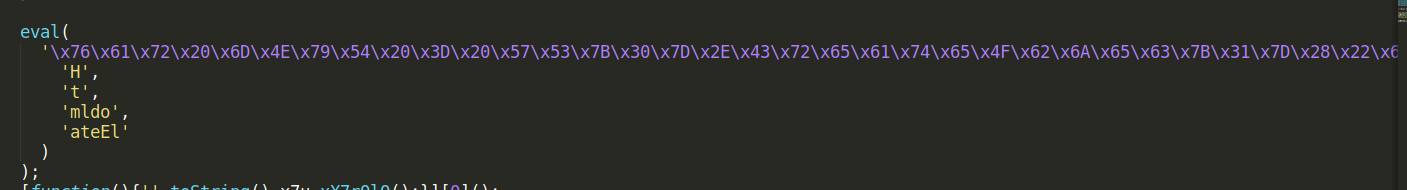
\includegraphics[width=15cm]{images/level2.png}
			\caption{Nivel 2: Hexadecimal Ofuscado} 
		\end{figure}
		
		\begin{figure}[H]
			\centering
			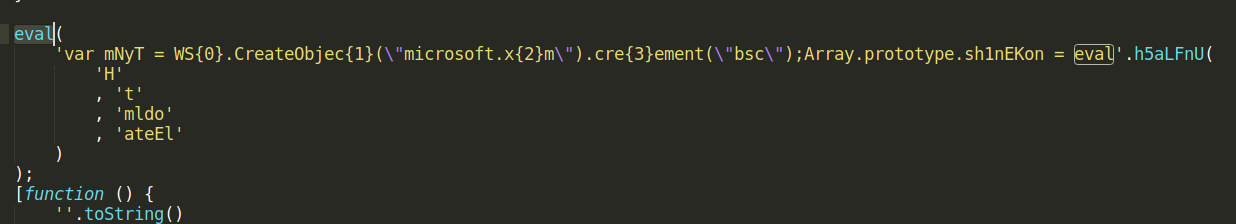
\includegraphics[width=15cm]{images/level2_after.png}
			\caption{Nivel 2: Hexadecimal Desofuscado} 
		\end{figure}
		
	
	\subsubsection{Ejemplo de Nivel 3: Parsear Unicodes}
	Para ello, se ha utilizado la librería \verb*|re| de Python, muy famosa para utilzar expresiones regulares. Se buscan los caracteres unicode que suelen ser 4 caracteres comenzando por \verb*|\u| y luego se parsean a String:
	\begin{scriptsize}
		\estiloR
		\begin{lstlisting}[caption={Desofuscación de ficheros JavaScript Nivel 3: Unicode}, language={python}]
		"""
Parse char unicode to char
		"""
		def parse_unicode(data):
def replace_unicode(match):
    return chr(int(match.group(1), 16))
		
pattern = r'\\u([0-9a-fA-F]{4})'
		
data = re.sub(pattern, replace_unicode, data)
		
return data
		
		\end{lstlisting}
	\end{scriptsize}
	
	\begin{scriptsize}
		\estiloR
		\begin{lstlisting}[caption={Desofuscación de ficheros JavaScript Nivel 3: Unicode}, language={bash}]
			python freyja.py -f ./samples/b122473d00566758d09c695d191b368e0c815c65e8acc0f00da7a88e45cc8a9e.js -l 3
		\end{lstlisting}
	\end{scriptsize}
	
	
	\begin{figure}[H]
		\centering
		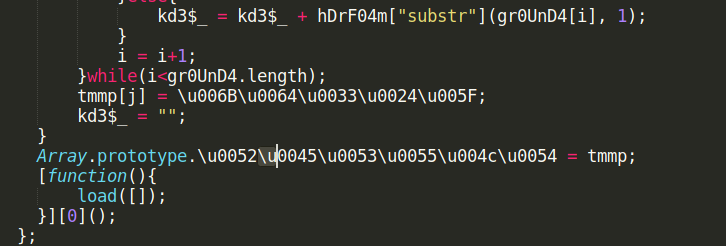
\includegraphics[width=10cm]{images/level3.png}
		\caption{Nivel 3: Unicode Ofuscado} 
	\end{figure}
	
	\begin{figure}[H]
		\centering
		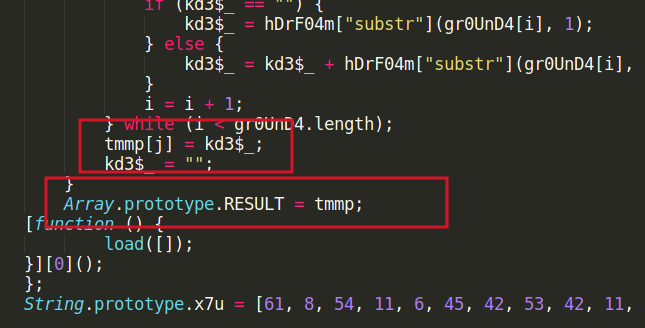
\includegraphics[width=10cm]{images/level3_after.png}
		\caption{Nivel 3: Unicode Desofuscado} 
	\end{figure}
	
	\subsubsection{Ejemplo de Nivel 4 y 5: Reemplazar la función toString}
	Para ello, se ha utilizado la librería \verb*|re| de Python, muy famosa para utilzar expresiones regulares. Se busca texto tipo \verb*|(23).toString(0x24)| o \verb*|(14).toString(36)|
	\begin{scriptsize}
		\estiloR
		\begin{lstlisting}[caption={Desofuscación de ficheros JavaScript Nivel 4 y 5: toString}, language={python}]

"""
    Replaces toString function parsing its contect to string integer equivalent
    after parsing the integer to the new base
"""
def replace_tostring(data):
    # Regular expression pattern to match (number).toString( number )
    pattern = r'\(\s*(\d+)\s*\)\s*\.toString\(\s*(\d+)\s*\)'

    # Find all matches of the pattern
    matches = re.finditer(pattern, data, re.MULTILINE)

    length = 0

    for match in matches:
        # Extract the two numbers from the matched groups
        first_number = int(match.group(1))
        second_number = int(match.group(2))

        to_string = numpy.base_repr(first_number, second_number)

        to_string = "\"" + to_string + "\""

        data = data[:match.start() - length] + to_string + data[match.end() - length:]

        length = length + len(match.group(0)) - 3

    return data


"""
    Replaces toString function parsing its contect to string integer equivalent
    after parsing the hex to integer and then to the new base
"""
def replace_hex_tostring(data):
    # Regular expression pattern to match (number).toString( number )
    pattern = r'\(\s*(\d+)\s*\)\s*\.toString\(\s*(0x[\da-fA-F]+)\s*\)'

    # Find all matches of the pattern
    matches = re.finditer(pattern, data, re.MULTILINE)

    length = 0

    for match in matches:
        # Extract the two numbers from the matched groups
        first_number = int(match.group(1))
        second_number = match.group(2)

        second_number = int(second_number, 16)

        to_string = numpy.base_repr(first_number, second_number)

        to_string = "\"" + to_string + "\""

        data = data[:match.start() - length] + to_string + data[match.end() - length:]

        length = length + len(match.group(0)) - 3

    return data

		
		\end{lstlisting}
	\end{scriptsize}
	
	\begin{scriptsize}
		\estiloR
		\begin{lstlisting}[caption={Desofuscación de ficheros JavaScript Nivel 4 y 5: toString}, language={bash}]
			python freyja.py -f ./samples/simple_js_malware_code/do_not_run.js -l 4
		\end{lstlisting}
	\end{scriptsize}
	
	
	\begin{figure}[H]
		\centering
		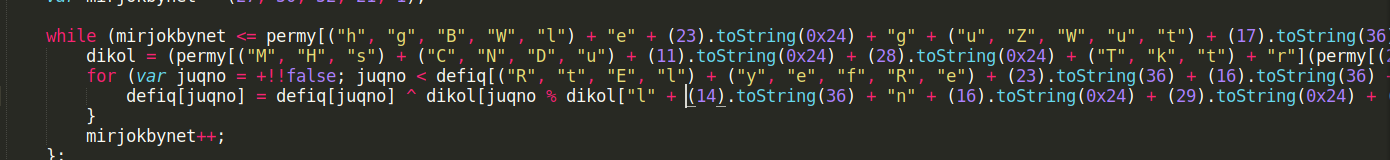
\includegraphics[width=15cm]{images/level4.png}
		\caption{Nivel 4 y 5: toString Ofuscado} 
	\end{figure}
	
	\begin{figure}[H]
		\centering
		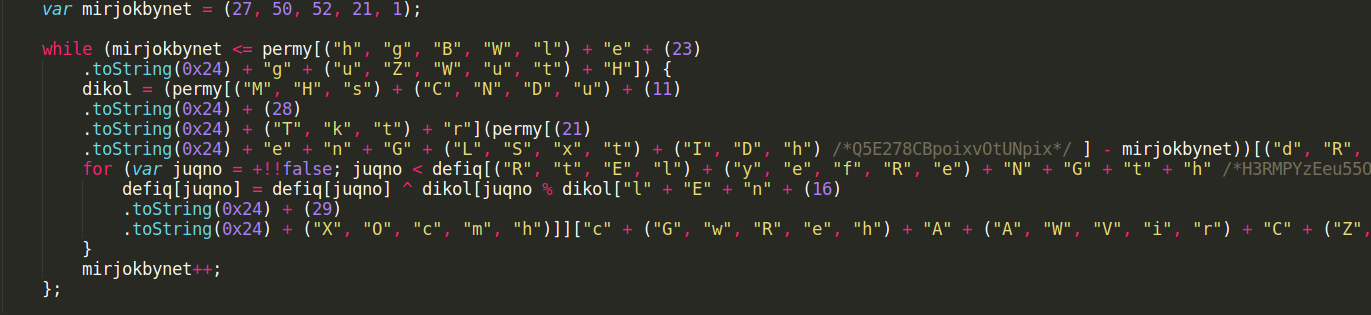
\includegraphics[width=15cm]{images/level4_after.png}
		\caption{Nivel 4: toString Desofuscado} 
	\end{figure}
	\begin{figure}[H]
		\centering
		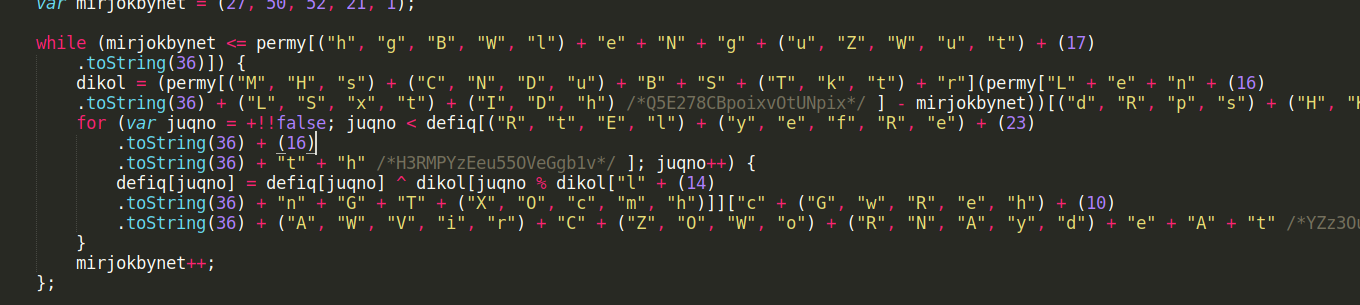
\includegraphics[width=15cm]{images/level5_after.png}
		\caption{Nivel 4: toString Hex Desofuscado} 
	\end{figure}
	
	\subsubsection{Ejemplo de Nivel 6: Parsear eval si tiene una lista de números}
	Para ello, se ha utilizado la librería \verb*|re| de Python, muy famosa para utilzar expresiones regulares. Se buscan listas de números como en la muestra extraída de un pdf \verb*|sample_2.js| que contiene una lista de números dentro de una expresión \verb*|eval|:
	
	\begin{scriptsize}
		\estiloR
		\begin{lstlisting}[caption={Desofuscación de ficheros JavaScript Nivel 6: Eval}, language={python}]
		"""
		    Replaces eval with a list of numbers
		"""
		def parse_eval_list_numbers(data):
		    def replace_with_chars(match):
		        numbers = re.findall(r'\d+', match.group(1))
		        chars = ''.join(chr(int(num)) for num in numbers)
		        return "\'" + chars + "\'"
		
		    pattern = r"'([^']*?\((?:\d+(?:\s*,\s*)?)+\))'"
		    data = re.sub(pattern, replace_with_chars, data)
		
		    return data
		
		
		\end{lstlisting}
	\end{scriptsize}
	
	\begin{scriptsize}
		\estiloR
		\begin{lstlisting}[caption={Desofuscación de ficheros JavaScript Nivel 6: Eval}, language={bash}]
			python freyja.py -f ./samples/sample_2_extracted/sample_2.js -l 6
		\end{lstlisting}
	\end{scriptsize}
	
	
	\begin{figure}[H]
		\centering
		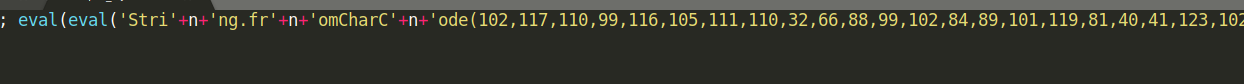
\includegraphics[width=15cm]{images/level6.png}
		\caption{Nivel 6: Eval Ofuscado} 
	\end{figure}
	
	\begin{figure}[H]
		\centering
		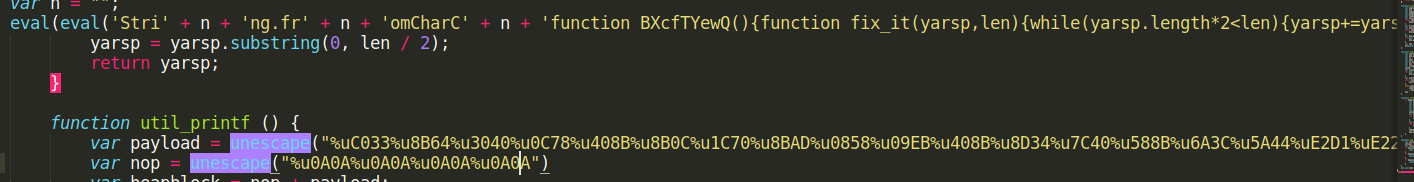
\includegraphics[width=15cm]{images/level6_after.png}
		\caption{Nivel 6: Eval Desofuscado} 
	\end{figure}
	

	\subsubsection{Ejemplo de Nivel 7: Parsear la función unescape}
	Para ello, se ha utilizado la librería \verb*|re| de Python, muy famosa para utilzar expresiones regulares. Se desofusca el texto que está en Unicode o en formato URL parseándolo a String:
	
	\begin{scriptsize}
		\estiloR
		\begin{lstlisting}[caption={Desofuscación de ficheros JavaScript Nivel 7: Eval}, language={python}]
		
		"""
		    Replaces unescape function parsing the content to string
		"""
		def parse_unescape(data):
		    pattern = r'unescape\([\'"]([^\'"]+)[\'"]\)'
		
		    def replacement(match):
		        unicode_escaped = urllib.parse.unquote(match.group(1))
		        replaced_unicode_escaped = unicode_escaped.replace('%', '\\')
		        decoded_string = bytes(replaced_unicode_escaped, 'utf-8').decode('unicode_escape')
		        return "\'" + decoded_string + "\'"
		
		    data = re.sub(pattern, replacement, data)
		    return data

				
		\end{lstlisting}
	\end{scriptsize}
	
	\begin{scriptsize}
		\estiloR
		\begin{lstlisting}[caption={Desofuscación de ficheros JavaScript Nivel 7: unescape}, language={bash}]
			python freyja.py -f ./samples/javascript-malware-collection/2016/20160311/20160311_01284d18e603522cc8bdabed57583bb3.js -l 7
		\end{lstlisting}
	\end{scriptsize}
	
	
	\begin{figure}[H]
		\centering
		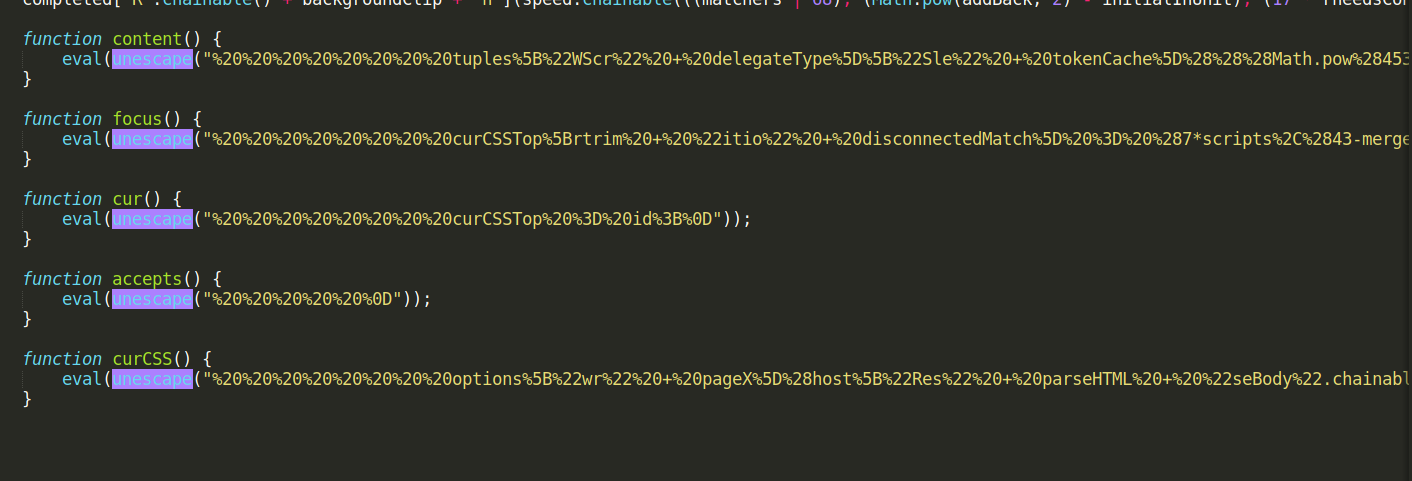
\includegraphics[width=15cm]{images/level7.png}
		\caption{Nivel 7: unescape Ofuscado} 
	\end{figure}
	
	\begin{figure}[H]
		\centering
		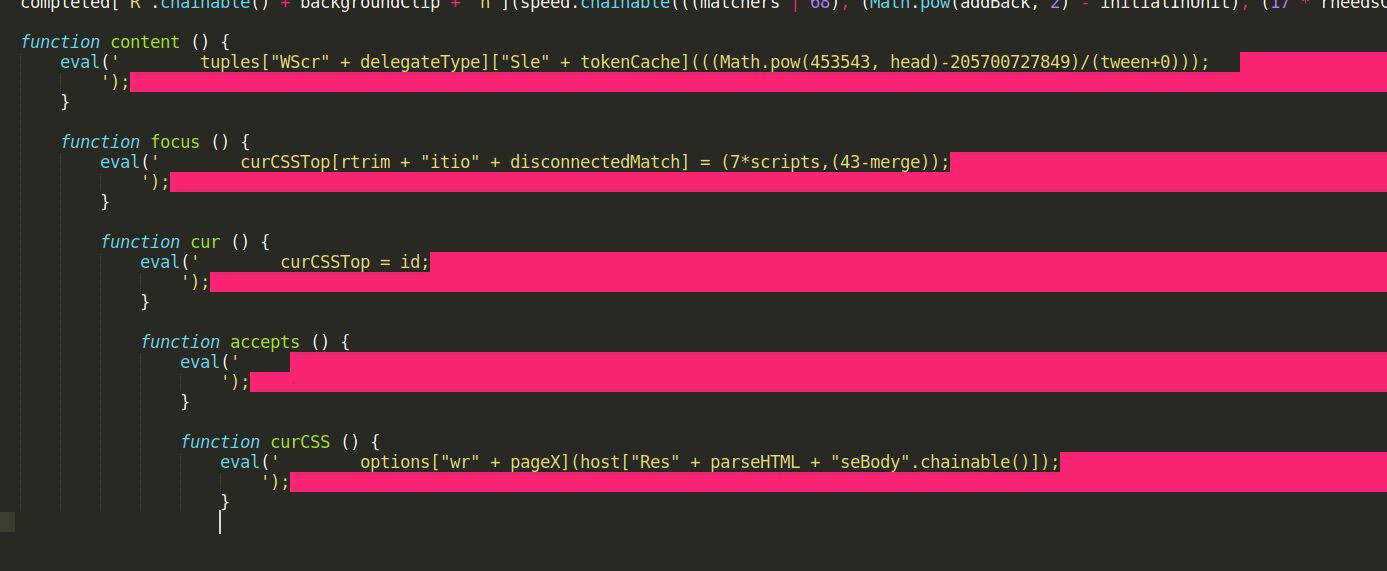
\includegraphics[width=15cm]{images/level7_after.png}
		\caption{Nivel 7: unescape Desofuscado} 
	\end{figure}
	
	
	\subsubsection{Ejemplo de Nivel 8: Parsear conjuntos de caracteres}
	Para ello, se ha utilizado la librería \verb*|re| de Python, muy famosa para utilzar expresiones regulares. Se buscan conjuntos de caracteres separados por \verb*|+|, ya que JavaScript sólo deja el último de la lista:
	
	\begin{scriptsize}
		\estiloR
		\begin{lstlisting}[caption={Desofuscación de ficheros JavaScript Nivel 8: Conjuntos de caracteres}, language={python}]
				
		
		"""
		    If there is a char set, it replaces it with the last value ("A", "B", "C") is "C"
		"""
		def parse_char_set(data):
		    pattern = r'\+\s*\((\s*"[a-zA-Z]"\s*,\s*)+\s*"([a-zA-Z])"\s*\)\s*\+'
		
		    # Find all matches of the pattern
		    matches = re.finditer(pattern, data, re.MULTILINE)
		
		    length = 0
		
		    for match in matches:
		        to_string = "+ \"" + match.group(2) + "\" +"
		        data = data[:match.start() - length] + to_string + data[match.end() - length:]
		
		        length = length + len(match.group(0)) - 7
		
		    pattern = r'\+\s*\((\s*"[a-zA-Z]"\s*,\s*)+\s*"([a-zA-Z])"\s*\)\s*'
		
		    # Find all matches of the pattern
		    matches = re.finditer(pattern, data, re.MULTILINE)
		
		    length = 0
		
		    for match in matches:
		        to_string = "+ \"" + match.group(2) + "\" "
		
		        data = data[:match.start() - length] + to_string + data[match.end() - length:]
		
		        length = length + len(match.group(0)) - 6
		
		    pattern = r'\s*\((\s*"[a-zA-Z]"\s*,\s*)+\s*"([a-zA-Z])"\s*\)\s*\+'
		
		    # Find all matches of the pattern
		    matches = re.finditer(pattern, data, re.MULTILINE)
		
		    length = 0
		
		    for match in matches:
		        to_string = " \"" + match.group(2) + "\" +"
		
		        data = data[:match.start() - length] + to_string + data[match.end() - length:]
		
		        length = length + len(match.group(0)) - 6
		
		    return data


		\end{lstlisting}
	\end{scriptsize}
	
	\begin{scriptsize}
		\estiloR
		\begin{lstlisting}[caption={Desofuscación de ficheros JavaScript Nivel 8: Conjuntos de caracteres}, language={bash}]
			python freyja.py -f freyja -f ./samples/simple_js_malware_code/do_not_run.js -l 8
		\end{lstlisting}
	\end{scriptsize}
	
	
	\begin{figure}[H]
		\centering
		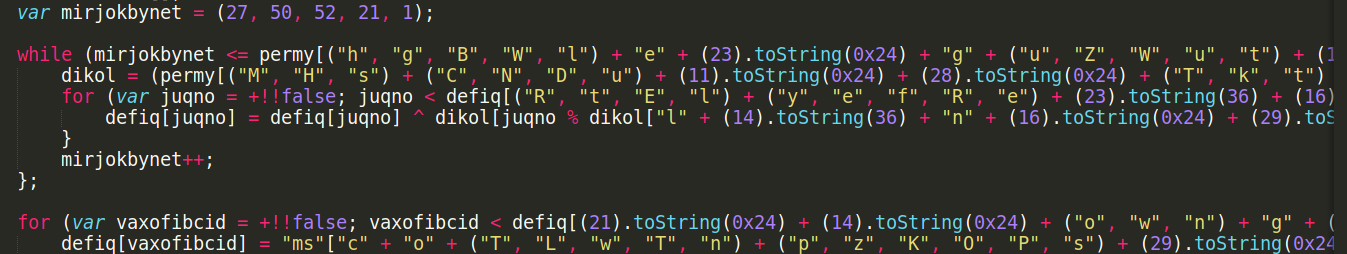
\includegraphics[width=12cm]{images/level8.png}
		\caption{Nivel 8: Conjuntos de caracteres Ofuscados} 
	\end{figure}
	
	\begin{figure}[H]
		\centering
		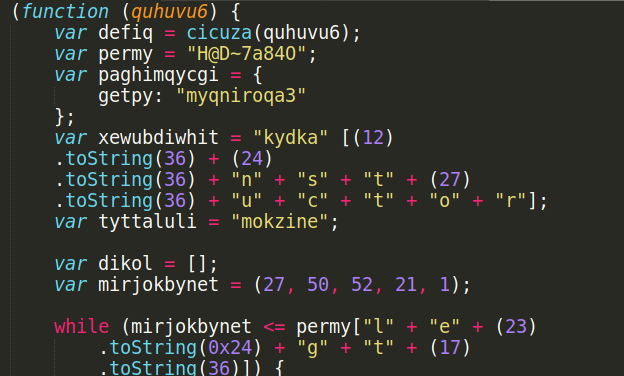
\includegraphics[width=10cm]{images/level8_after.png}
		\caption{Nivel 8: Conjuntos de caracteres Desofuscados} 
	\end{figure}
	
	
	\subsubsection{Ejemplo de Nivel 9: Parsear la función parseInt}
	Para ello, se ha utilizado la librería \verb*|re| de Python, muy famosa para utilzar expresiones regulares. Se desofusca pasando a entero el parámetro de la función. En este caso reutilizamos la salida del nivel 4 \verb*|out.js|:
	
	\begin{scriptsize}
		\estiloR
		\begin{lstlisting}[caption={Desofuscación de ficheros JavaScript Nivel 9: parseInt}, language={python}]
		
		"""
		    Replaces parseInt function parsing the content char to a in integer value
		"""
		def parse_int(data):
		    pattern = r'parseInt\("(\d+)"\)'
		
		    # Find all matches of the pattern
		    matches = re.finditer(pattern, data, re.MULTILINE)
		
		    length = 0
		
		    for match in matches:
		        data = data[:match.start() - length] + match.group(1) + data[match.end() - length:]
		
		        length = length + len(match.group(0)) - 1
		
		    return data
		

				
		\end{lstlisting}
	\end{scriptsize}
	
	\begin{scriptsize}
		\estiloR
		\begin{lstlisting}[caption={Desofuscación de ficheros JavaScript Nivel 9: parseInt}, language={bash}]
			python freyja.py -f out.js -l 9
		\end{lstlisting}
	\end{scriptsize}
	
	
	\begin{figure}[H]
		\centering
		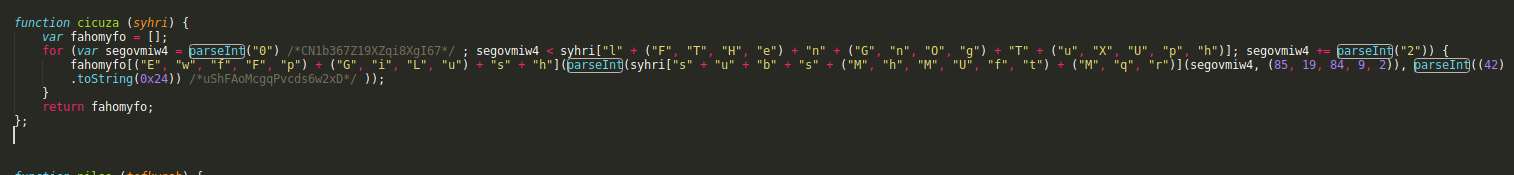
\includegraphics[width=18cm]{images/level9.png}
		\caption{Nivel 9: parseInt Ofuscado} 
	\end{figure}
	
	\begin{figure}[H]
		\centering
		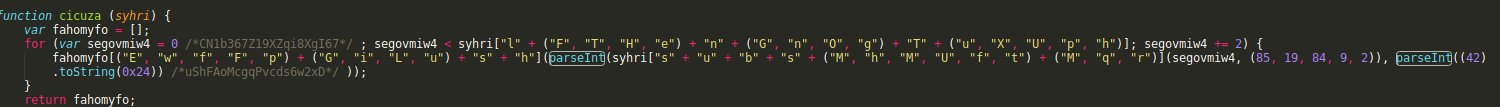
\includegraphics[width=18cm]{images/level9_after.png}
		\caption{Nivel 9: parseInt Desofuscado} 
	\end{figure}

	\subsubsection{Ejemplo de Nivel 10: Parsear las concatenaciones de caracteres}
	Para ello, se ha utilizado la librería \verb*|re| de Python, muy famosa para utilzar expresiones regulares. Se concatenan todos los caracteres separados por \verb*|+|. Para el ejemplo reutilizaremos el \verb*|out.js|:
	
	\begin{scriptsize}
		\estiloR
		\begin{lstlisting}[caption={Desofuscación de ficheros JavaScript Nivel 10: Concatenación}, language={python}]

		
		"""
		    Appending characrers between + like "A" + "B" 
		"""
		def append_strings_multi(data):
		    # Regular expression pattern to match (number).toString( number )
		    pattern = r'[\'\"]\s+\+\s+[\'\"]'
		
		    # Find all matches of the pattern
		    matches = re.finditer(pattern, data, re.MULTILINE)
		
		    length = 0
		
		    for match in matches:
		
		        to_string = ""
		
		        data = data[:match.start() - length] + to_string + data[match.end() - length:]
		
		        length = length + len(match.group(0))
		
		    return data
		

		\end{lstlisting}
	\end{scriptsize}
	
	\begin{scriptsize}
		\estiloR
		\begin{lstlisting}[caption={Desofuscación de ficheros JavaScript Nivel 10: Concatenación}, language={bash}]
			python freyja.py -f out.js -l 10
		\end{lstlisting}
	\end{scriptsize}
	
	
	\begin{figure}[H]
		\centering
		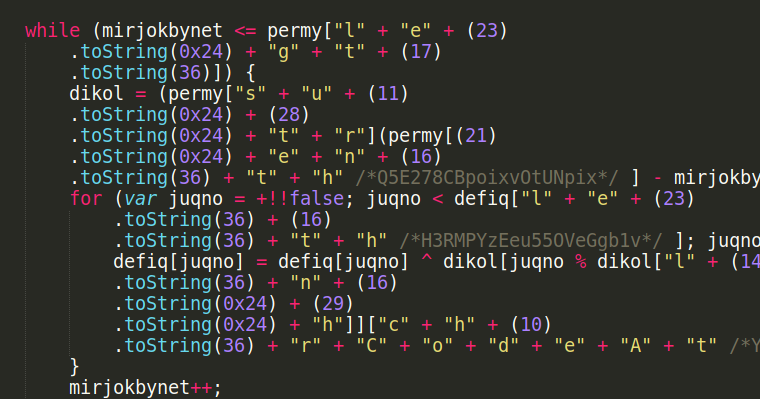
\includegraphics[width=12cm]{images/level10.png}
		\caption{Nivel 10: Concatenación Ofuscada} 
	\end{figure}
	
	\begin{figure}[H]
		\centering
		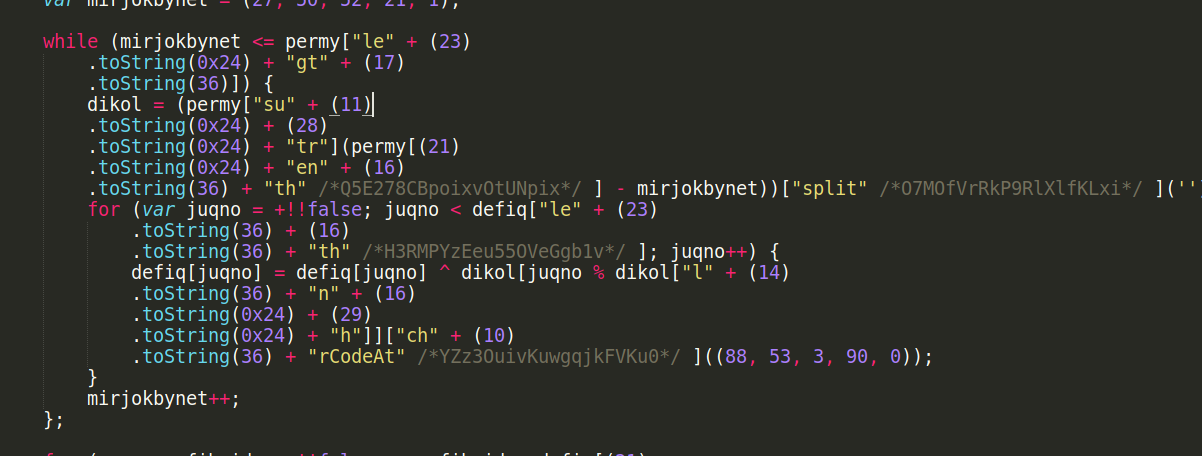
\includegraphics[width=12cm]{images/level10_after.png}
		\caption{Nivel 10: Concatenación Desofuscada} 
	\end{figure}
	
	\subsection{Búsquedas de Base64}
	Esta herramienta también puede buscar y decodificar strings de Base64 en un fichero de texto. Para ello utiliza la librería librería \verb*|re| de Python para buscar con la expresión regular referente a strings codificados en Base64:


	\begin{scriptsize}
		\estiloR
		\begin{lstlisting}[caption={Búsqueda de Base64}, language={python}]

		
		"""
		    Finds base64 between '' and "" and then deletes first and last character 
		"""
		def find_base64(data):
		    base64_pattern = r'["\'](?:[A-Za-z0-9+/]{4})*(?:[A-Za-z0-9+/]{2}==|[A-Za-z0-9+/]{3}=|[A-Za-z0-9+/]{4})["\']'
		    base64_strings = re.findall(base64_pattern, data)
		
		    base64_strings_cleaned = []
		    for match in base64_strings:
		        match = match[1:-1]
		        if len(match) >= 10:
		            base64_strings_cleaned.append(match)
		    return base64_strings_cleaned
		
		"""
		    Decodes base64 and saves it to json output file
		"""
		def decode_base64(encoded_data):
		    decoded_strings = []
		    for base64_string in encoded_data:
		        decoded_bytes = base64.b64decode(base64_string)
		        try:
		            decoded_string = decoded_bytes.decode("'utf-8'")
		        except UnicodeDecodeError:
		            decoded_string = decoded_bytes.decode("iso-8859-1")
		
		        decoded_dict = {'original': base64_string, 'decoded':decoded_string}
		        decoded_strings.append(decoded_dict)
		    return decoded_strings
		
		

		\end{lstlisting}
	\end{scriptsize}
	
	\begin{scriptsize}
		\estiloR
		\begin{lstlisting}[caption={Búsqueda de Base64}, language={bash}]
			python freyja.py -b example.txt -o example.json
		\end{lstlisting}
	\end{scriptsize}
	
	
	\begin{figure}[H]
		\centering
		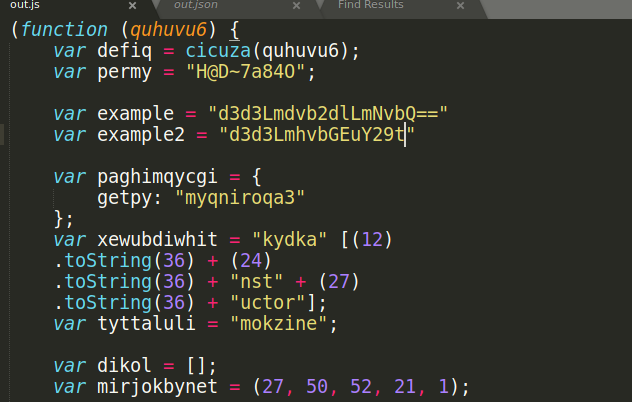
\includegraphics[width=12cm]{images/base64_before.png}
		\caption{Búsqueda de Base64 Ofuscada} 
	\end{figure}
	
	\begin{figure}[H]
		\centering
		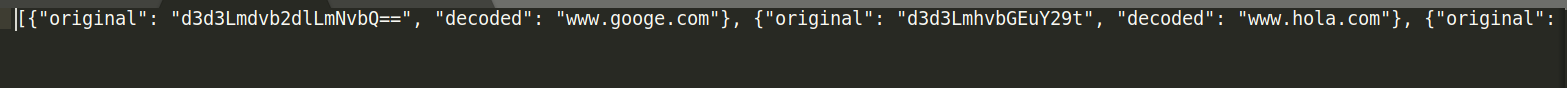
\includegraphics[width=18cm]{images/base64_after.png}
		\caption{Búsqueda de Base64 Desofuscada} 
	\end{figure}

	\section{Video Tutorial}
	\href{https://www.mediafire.com/file/pqmjs5vcqf3jvau/tutorial.mkv/file}{https://www.mediafire.com/file/pqmjs5vcqf3jvau/tutorial.mkv/file}
	
	\newpage
	\listoffigures
	\lstlistoflistings
	\newpage
	\section{Bibliografía}
	\begin{thebibliography}{40}
		\bibitem{introduction}
		Técnicas más comunes de ofuscación
		
		\href{https://www.socinvestigation.com/most-common-malware-obfuscation-techniques/}{https://www.socinvestigation.com/most-common-malware-obfuscation-techniques/}
		
		\bibitem{introduction2}
		Técnicas más comunes de ofuscación
		
		\href{https://minerva-labs.com/blog/malware-evasion-techniques-obfuscated-files-and-information/}{https://minerva-labs.com/blog/malware-evasion-techniques-obfuscated-files-and-information/}
		
		\bibitem{yara}
		Reglas Yara en VirusTotal
		
		\href{https://virustotal.github.io/yara/}{https://virustotal.github.io/yara/}
		
		\bibitem{polymorfic}
		Malware Polimórfico
		
		\href{https://ayudaleyprotecciondatos.es/2021/04/29/malware-polimorfico/}{https://ayudaleyprotecciondatos.es/2021/04/29/malware-polimorfico/}
		
		\bibitem{techniques}
		Metamorphic Malware and Obfuscation -A Survey of Techniques, Variants and Generation Kits
		
		\href{https://www.researchgate.net/publication/357255382_Metamorphic_Malware_and_Obfuscation_-A_Survey_of_Techniques_Variants_and_Generation_Kits}{https://www.researchgate.net/}
		
		\bibitem{parasite}
		Crafting a peaceful parasite
		
		\href{https://compilepeace.medium.com/malware-engineering-part-0x3-crafting-a-peaceful-parasite-c8c6c9a0b010}{https://compilepeace.medium.com}
		
		\bibitem{mba}
		h-c0n2020 Arnau Gámez Code obfuscation through Mixed Boolean-Arithmetic expressions
		
		\href{https://github.com/arnaugamez/talks/blob/main/2022/00_h-c0n/slides.pdf}{https://github.com/arnaugamez/}
		
		
		\bibitem{virustotal}
		Página de búsqueda de malware por su hash Virus Total
		
		\href{https://www.virustotal.com/gui/home/upload}{https://www.virustotal.com/}
		
		\bibitem{redlinestealer}
		Redline Stealer
		
		\href{https://minerva-labs.com/blog/redline-stealer-masquerades-as-telegram-installer/}{https://minerva-labs.com/}
		
		\bibitem{hancitor}
		Malware Hancitor
		
		\href{https://minerva-labs.com/blog/hancitor-malware/}{https://minerva-labs.com/}
		
		\bibitem{regswap}
		Malware W95/Regswap
		
		\href{https://www.microsoft.com/en-us/wdsi/threats/malware-encyclopedia-description?Name=Virus:Win95/Regswap.1644.dr&threatId=-2147420803}{https://www.microsoft.com/}
		
		
		\bibitem{zmist}
		Malware W95/Zmist
		
		\href{https://www.microsoft.com/en-us/wdsi/threats/malware-encyclopedia-description?Name=Virus%3AWin95%2FZmist.A&ThreatID=-21474218163}{https://www.microsoft.com/}
		
		\bibitem{metaphor}
		Malware MetaPHOR
		
		\href{http://virus.wikidot.com/metaphor}{http://virus.wikidot.com/}
		
		\bibitem{zperm}
		Malware Win32/Zperm
		
		\href{https://www.microsoft.com/en-us/wdsi/threats/malware-encyclopedia-description?Name=Virus:Win32/Zperm.A}{https://www.microsoft.com/}
		
		\bibitem{avron}
		Gusano Lirva, alias Avron
		
		\href{https://unaaldia.hispasec.com/2003/01/versiones-del-gusano-lirva-alias-avril-avron-naith.html}{https://unaaldia.hispasec.com/}
		
		\bibitem{whale}
		Malware Whale DOS
		
		\href{https://en.wikipedia.org/wiki/Whale_(computer_virus)}{https://en.wikipedia.org/}
		
		\bibitem{memorial}
		Malware Win95/Memorial
		
		\href{https://threats.kaspersky.com/mx/threat/Virus.Win9x.Memorial/}{https://threats.kaspersky.com/}
		
		\bibitem{1260}
		Malware 1260 o V2PX
		
		\href{https://en.wikipedia.org/wiki/1260_(computer_virus)}{https://en.wikipedia.org/}
		
		\bibitem{psmpc}
		Herramienta PS-MPC de ofuscación de malware polimórfico
		
		\href{https://www.f-secure.com/v-descs/ps-mpc.shtml}{https://www.f-secure.com/v-descs/ps-mpc.shtml}
		
		\bibitem{vcl}
		Herramienta PS-MPC de ofuscación de malware polimórfico
		
		\href{https://threats.kaspersky.com/en/threat/Constructor.DOS.VCL/}{https://threats.kaspersky.com/}
		
		\bibitem{vienna}
		Malware Vienna
		
		\href{https://www.f-secure.com/v-descs/vienna.shtml}{https://www.f-secure.com/v-descs/vienna.shtml}
		
		\bibitem{luna}
		Luna, el primer malware polimórfico de la historia.
		
		\href{http://virus.wikidot.com/luna#toc2}{http://virus.wikidot.com/}
		
		\bibitem{loveletter}
		Gusano	LoveLetter o ILOVEYOU
		\href{https://threats.kaspersky.com/mx/threat/Email-Worm.VBS.LoveLetter/}{https://threats.kaspersky.com/}
		
		\bibitem{stormwormemail}
		Gusano Storm Worm
		
		\href{https://www.hellotech.com/blog/storm-worm-malware}{https://www.hellotech.com/blog/storm-worm-malware}
		
		\bibitem{cryptowall}
		Ransomware CryptoWall
		
		\href{https://www.pcrisk.es/guias-de-desinfeccion/7401-cryptowall-virus}{https://www.pcrisk.es/guias-de-desinfeccion/7401-cryptowall-virus}
		
		
		\bibitem{virlock}
		Ransomware Win32/VirLock
		
		\href{https://www.welivesecurity.com/la-es/2014/12/22/virlock-primer-ransomware-reproduce/}{https://www.welivesecurity.com/}
		
		
		\bibitem{cryptowall}
		Ransomware CryptoWall
		
		\href{https://www.pcrisk.es/guias-de-desinfeccion/7401-cryptowall-virus}{https://www.pcrisk.es/guias-de-desinfeccion/7401-cryptowall-virus}
		
		\bibitem{cryptxxx}
		Ransomware CryptXXX
		
		\href{https://www.pcrisk.es/guias-de-desinfeccion/8250-cryptxxx-ransomware}{https://www.pcrisk.es/guias-de-desinfeccion/8250-cryptxxx-ransomware}
		
		\bibitem{cryptolocker}
		Ransomware CryptoLocker
		
		\href{https://www.avast.com/es-es/c-cryptolocker}{https://www.avast.com/es-es/c-cryptolocker}
		
		\bibitem{wannacry}
		Ransomware WannaCry
		
		\href{https://www.kaspersky.es/resource-center/threats/ransomware-wannacry}{https://www.kaspersky.es/}
		
		\bibitem{ghost}
		Ransomware Ghost
		
		\href{https://www.malwarerid.com/malwares/el-ransomware-ghost}{https://www.malwarerid.com/malwares/el-ransomware-ghost}
		
		\bibitem{ngvck}
		Troyano Win32/NGVCK
		
		\href{https://www.microsoft.com/en-us/wdsi/threats/malware-encyclopedia-description?Name=Trojan:Win32/Ngvck!mclg&threatId=-2147180992}{https://www.microsoft.com/}
		
		\bibitem{etap}
		Malware W32/Etap
		
		\href{https://threats.kaspersky.com/mx/threat/Virus.Win32.Etap/}{https://threats.kaspersky.com/}
		
		\bibitem{cascade}
		Malware Cascade
		
		\href{https://en.wikipedia.org/wiki/Cascade_(computer_virus)}{https://en.wikipedia.org/}
		
		\href{https://gist.github.com/RC1140/5183430}{github Source code}
		
		\bibitem{upx}
		UPX Packer
		
		\href{https://upx.github.io/}{https://upx.github.io/}
		
		\bibitem{aspack}
		ASPACK Packer
		
		\href{http://www.aspack.com/}{http://www.aspack.com/}
		
		\bibitem{shannon1}
		Algoritmo de Shannon
		
		\href{https://gist.github.com/nstarke/bc662d2858756f4812d74f7fb3eab28a}{https://gist.github.com/nstarke/bc662d2858756f4812d74f7fb3eab28a}
		
		\bibitem{obfuscationbible}
		PowerShell Obfuscation Bible
		
		\href{https://github.com/t3l3machus/PowerShell-Obfuscation-Bible#Randomize-Char-Cases}{https://github.com/t3l3machus/}
		
		\bibitem{javascript_malware}
		Understanding the Windows JavaScript Threat Landscape:
		
		\href{https://www.deepinstinct.com/blog/understanding-the-windows-javascript-threat-landscape}{https://www.deepinstinct.com/blog/understanding-the-windows-javascript-threat-landscape}
		
		\bibitem{cobalstrike}
		Cobalt Strike
		
		\href{https://www.cobaltstrike.com/}{https://www.cobaltstrike.com/}
		
		\bibitem{jsmalwareobfuscation}
		Understanding JavaScript Malware Obfuscation
		
		\href{https://github.com/bl4de/research/blob/master/javascript-malware-obfuscation/Simple_JavaScript_malware_code_obfuscation_examples.md}{https://github.com/bl4de/research/tree/master/javascript-malware-obfuscation}
		
		\bibitem{wshrat}
		Analizando la ofuscación de WSHRAT (VB)
		\href{https://www.binarydefense.com/resources/blog/revenge-is-a-dish-best-served-obfuscated/}{https://www.binarydefense.com/}
				
		
	\end{thebibliography}



\end{document}